\documentclass[aspectratio=169]{beamer}

\mode<presentation> {
\usetheme{Madrid}
}

\usepackage{graphicx}
\usepackage{booktabs}

\title[To study Linux and Hardware with QEMU]{To study Linux and Hardware with QEMU}

\author{Dongli Zhang}
\date{\today}

\begin{document}

%------------------------------------------------

\section{Title}
\begin{frame}
\titlepage
\end{frame}

%------------------------------------------------

\section{When to study and debug SCSI ...}
\begin{frame}
\frametitle{When to study and debug SCSI ...}
\Large When to study the concept of SCSI \textcolor{red}{$<$adapter, channel, id, lun$>$} ...
\begin{itemize}
\visible<1->{\item There is \textcolor{red}{no} SCSI hardware available}
\visible<1->{\item To reboot the test server is \textcolor{red}{time-consuming}}
\visible<1->{\item It is hard to customize \textcolor{red}{SCSI topology} (e.g., \#lun or \#target)}
\visible<1->{\item It is hard to customize \textcolor{red}{SCSI config} (e.g., \#queue for mq)}
\end{itemize}
\end{frame}

%------------------------------------------------

\section{SCSI is not the end ...}
\begin{frame}
\frametitle{SCSI is not the end ...}
{\LARGE We may want to study more \textbf{\textcolor{blue}{Linux and Hardware features}}...}
\begin{columns}[c]
\column{.45\textwidth}
{ \Large
\begin{itemize}
\item SCSI
\item NVMe
\item NVDIMM
\item Virtio
\item Ethernet
\item PCI and PCIe
\end{itemize}
}
\column{.45\textwidth}
{ \Large
\begin{itemize}
\item BIOS
\item IOMMU
\item NUMA
\item CPU Hotplug
\item Memroy Hotplug
\item PM Suspend
\end{itemize}
}
\end{columns}
\end{frame}

%------------------------------------------------

\section{Why QEMU}
\begin{frame}
\frametitle{Why QEMU}
\large
QEMU is a generic and open source machine emulator and virtualizer
\begin{itemize}
\item QEMU can emulate lots of hardware
\item \textcolor{red}{QEMU can boot from Linux kernel on host}
    \begin{itemize}
	\item It is time-consuming to build and install kernel in VM
    \end{itemize}
\end{itemize}

This tutorial is \textbf{\textcolor{blue}{NOT}} to...
\begin{itemize}
\item teach how to use QEMU cmdline
\item \textcolor{red}{how to build and debug kernel inside guest}
\item how to debug generic features like buddy allocator or CFS scheduler
\item how to debug advanced features (e.g., qlogic) with QEMU
\item what is SCSI, NVMe, NVDIMM ...
\end{itemize}			
\end{frame}

%------------------------------------------------

\section{Build QEMU and Guest Linux}
\begin{frame}
\frametitle{Build QEMU and Guest Linux}
\begin{itemize}
\item {\Large QEMU version in the tutorial: commit \textbf{\textcolor{olive}{076243ffe6c1}}}
\item {\Large Linux version in the tutorial: tag \textbf{\textcolor{olive}{v5.2-rc4}}}
\end{itemize}
\begin{columns}[c]
\column{.45\textwidth}
\begin{block}{}
{ \small
To build Linux on host (All CONFIG is 'Y'):

\textcolor{red}{\# make defconfig}

\textcolor{red}{\# make menuconfig}

\textcolor{red}{\# make -j8 $>$ /dev/null} \newline

The output is something like:

\textbf{\textcolor{blue}{/.../linux/arch/x86\_64/boot/bzImage}}
}
\end{block}
\column{.45\textwidth}
\begin{block}{}
{ \small
To build QEMU:

\textcolor{red}{\# ./configure --target-list=x86\_64-softmmu}

\textcolor{red}{\# make -j8 $>$ /dev/null} \newline

We directly use output w/o 'make install':

\textbf{\textcolor{blue}{./x86\_64-softmmu/qemu-system-x86\_64}}
}
\end{block}
\end{columns}
\end{frame}

%------------------------------------------------

\section{Boot QEMU and Guest Linux}
\begin{frame}
\frametitle{Build QEMU and Guest Linux}
\begin{itemize}
\item No need to work with guest IP, but only \textbf{\textcolor{blue}{$<$host\_ip$>$:5022}}
\item Connect to guest via \textbf{\textcolor{blue}{VNC}}
\item Serial console output is redirected to \textbf{\textcolor{blue}{stdio}}
\end{itemize}
\begin{block}{}

To boot guest with Linux kernel locating on host:

\textcolor{red}{\# qemu-system-x86\_64 -machine accel=kvm \textbf{\textcolor{blue}{-vnc :0 -serial stdio}} -smp 4 -m 4096M} \textbackslash

\textcolor{red}{-net nic -net user,\textbf{\textcolor{blue}{hostfwd=tcp::5022-:22}}} \textbackslash

\textcolor{red}{-kernel /home/user/linux/arch/x86\_64/boot/bzImage} \textbackslash
	
\textcolor{red}{-append "root=/dev/sda1 init=/sbin/init text \textbf{\textcolor{blue}{console=ttyS0}}"} \textbackslash

\textcolor{red}{-hda /home/user/img/boot.qcow2} \newline

To login to guest in another shell:

\textcolor{red}{\# ssh user@$<$host\_ip$>$ -p 5022}

or

\textcolor{red}{\# vncviewer $<$host\_ip$>$}

\end{block}
\end{frame}

%------------------------------------------------

\section{SeaBIOS 1/2}
\begin{frame}
\frametitle{SeaBIOS 1/2}
\begin{itemize}
\item {\Large SeaBIOS is the default BIOS for QEMU and KVM}
\item {\Large https://git.seabios.org/seabios.git}
\item {\Large SeaBIOS version for the tutorial: commit \textbf{\textcolor{olive}{6e56ed129c97}}}
\end{itemize}
\begin{columns}[c]
\column{.45\textwidth}
\begin{block}{}
{
The below options are enabled to dump debug message to serial port: \newline

\textcolor{red}{CONFIG\_DEBUG\_LEVEL=8}

\textcolor{red}{CONFIG\_DEBUG\_SERIAL=y}

\textcolor{red}{CONFIG\_DEBUG\_SERIAL\_PORT=0x3f8}

\textcolor{red}{CONFIG\_DEBUG\_IO=y}

}
\end{block}
\column{.45\textwidth}
\begin{block}{}
{
To build SeaBIOS:

\textcolor{red}{\# make menuconfig}

\textcolor{red}{\# make} \newline

The output is at:

\textcolor{red}{/.../seabios/out/bios.bin}
}
\end{block}
\end{columns}
\end{frame}

%------------------------------------------------

\section{SeaBIOS 2/2}
\begin{frame}
\frametitle{SeaBIOS 2/2}
{ \LARGE \textbf{\textcolor{blue}{-serial stdio}} is used to dump debug message to stdio}
\begin{block}{}

To boot guest with Linux kernel and BIOS: \newline

\# qemu-system-x86\_64 -machine accel=kvm -vnc :0 -smp 4 -m 4096M \textbackslash

-net nic -net user,hostfwd=tcp::5022-:22 \textbackslash

-kernel /home/user/linux/arch/x86\_64/boot/bzImage \textbackslash
	
-append "root=/dev/sda1 init=/sbin/init text" \textbackslash

-hda /home/user/img/boot.qcow2 \textbackslash

\textcolor{red}{\textbf{\textcolor{blue}{-bios}} /home/user/seabios/out/bios.bin \textbf{\textcolor{blue}{-serial stdio}}}

\end{block}
\end{frame}

%------------------------------------------------

\section{SCSI: megasas 1/2}
\begin{frame}
\frametitle{SCSI: megasas 1/2}
{\LARGE 2 targets (each with a lun) on the same $<$adapter, channel$>$}
\\
%\begin{block}{two adapters (each with a lun) on the same $<$adapter, channel$>$}
\begin{block}{}

\# qemu-system-x86\_64 -machine accel=kvm -vnc :0 -smp 4 -m 4096M \textbackslash

-net nic -net user,hostfwd=tcp::5022-:22 \textbackslash

-kernel /home/user/linux/arch/x86\_64/boot/bzImage \textbackslash
	
-append "root=/dev/sda1 init=/sbin/init text" \textbackslash

\textcolor{red}{-device \textbf{\textcolor{blue}{megasas}},id=scsi0} \textbackslash

\textcolor{red}{-device scsi-hd,drive=drive0,\textbf{\textcolor{blue}{bus=scsi0.0,channel=0,scsi-id=0,lun=0}},bootindex=1} \textbackslash
 
\textcolor{red}{-drive file=/home/user/img/boot.qcow2,if=none,id=drive0} \textbackslash

\textcolor{red}{-device scsi-hd,drive=drive1,\textbf{\textcolor{blue}{bus=scsi0.0,channel=0,scsi-id=1,lun=0}}} \textbackslash

\textcolor{red}{-drive file=/home/user/img/disk.qcow2,if=none,id=drive1}

\end{block}
\end{frame}

%------------------------------------------------

\section{SCSI: megasas 2/2}
\begin{frame}
\frametitle{SCSI: megasas 2/2}
\begin{figure}
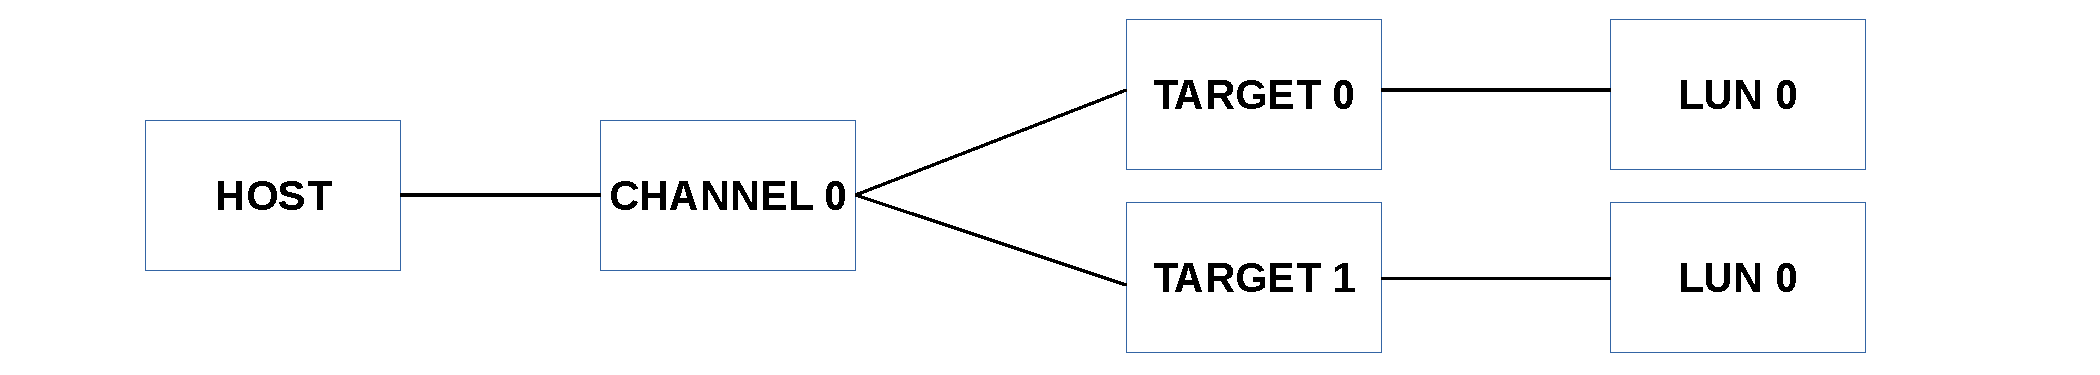
\includegraphics[width=1.0\linewidth]{figures/megasas.pdf}
\end{figure}
\begin{block}{}
[    0.626341] scsi host0: \textbf{\textcolor{blue}{Avago SAS based MegaRAID driver}}

[    0.644708] scsi \textcolor{red}{0:2:0:0}: Direct-Access     QEMU     QEMU HARDDISK    2.5+ PQ: 0 ANSI: 5

[    0.646012] scsi \textcolor{red}{0:2:1:0}: Direct-Access     QEMU     QEMU HARDDISK    2.5+ PQ: 0 ANSI: 5

[    0.671123] sd \textcolor{red}{0:2:0:0}: Attached scsi generic sg0 type 0

[    0.671710] sd \textcolor{red}{0:2:1:0}: Attached scsi generic sg1 type 0

[    0.673409] sd \textcolor{red}{0:2:1:0}: [sdb] Attached SCSI disk

[    0.680489] sd \textcolor{red}{0:2:0:0}: [sda] Attached SCSI disk
\end{block}
\end{frame}

%------------------------------------------------

\section{SCSI: lsi53c895a 1/2}
\begin{frame}
\frametitle{SCSI: lsi53c895a 1/2}
{\LARGE 2 targets (each with a lun) on the same $<$adapter, channel$>$}
\\
%{\Large 2 adapters (each with a lun) on the same $<$adapter, channel$>$}
\begin{block}{}

\# qemu-system-x86\_64 -machine accel=kvm -vnc :0 -smp 4 -m 4096M \textbackslash

-net nic -net user,hostfwd=tcp::5022-:22 \textbackslash

-kernel /home/user/linux/arch/x86\_64/boot/bzImage \textbackslash
	
-append "root=/dev/sda1 init=/sbin/init text" \textbackslash

\textcolor{red}{-device \textbf{\textcolor{blue}{lsi53c895a}},id=scsi0} \textbackslash
	
\textcolor{red}{-device scsi-hd,drive=drive0,\textbf{\textcolor{blue}{bus=scsi0.0,channel=0,scsi-id=0,lun=0}},bootindex=1} \textbackslash

\textcolor{red}{-drive file=/home/user/img/boot.qcow2,if=none,id=drive0} \textbackslash

\textcolor{red}{-device scsi-hd,drive=drive1,\textbf{\textcolor{blue}{bus=scsi0.0,channel=0,scsi-id=1,lun=0}}} \textbackslash

\textcolor{red}{-drive file=/home/user/img/disk.qcow2,if=none,id=drive1}
\end{block}
\end{frame}

%------------------------------------------------

\section{SCSI: lsi53c895a 2/2}
\begin{frame}
\frametitle{SCSI: lsi53c895a 2/2}
\begin{figure}
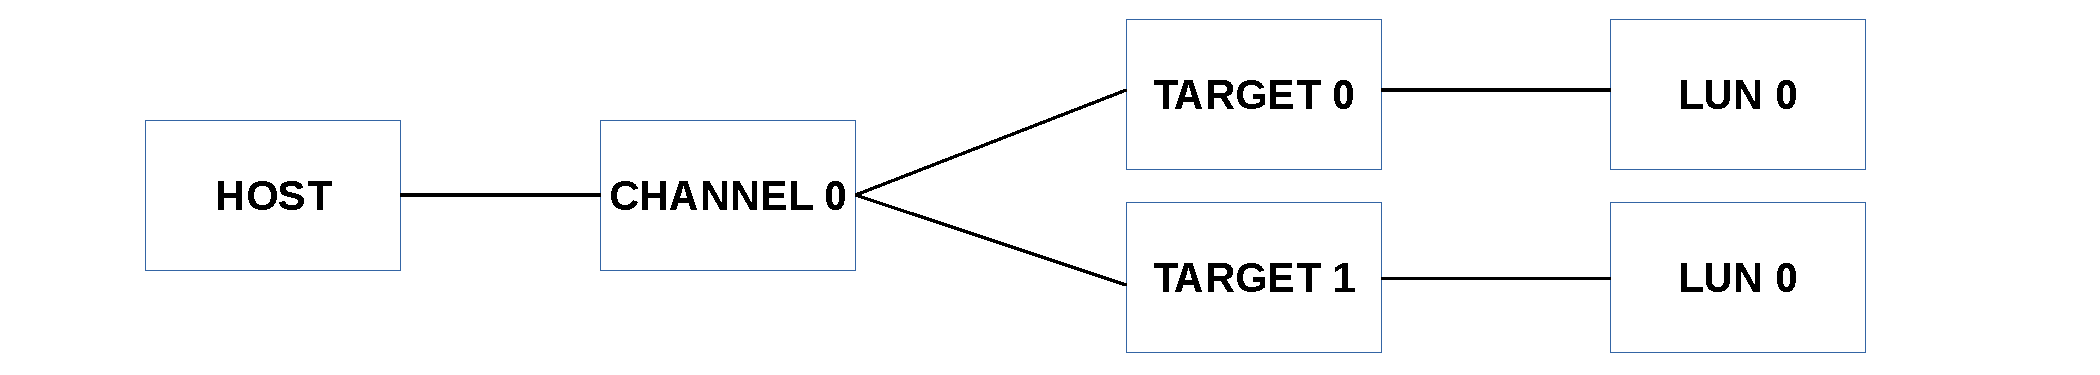
\includegraphics[width=1.0\linewidth]{figures/megasas.pdf}
\end{figure}
\begin{block}{}
[    0.610488] scsi host0: \textbf{\textcolor{blue}{sym-2.2.3}}

[    3.603414] scsi \textcolor{red}{0:0:0:0}: Direct-Access     QEMU     QEMU HARDDISK    2.5+ PQ: 0 ANSI: 5

[    3.613141] scsi \textcolor{red}{0:0:1:0}: Direct-Access     QEMU     QEMU HARDDISK    2.5+ PQ: 0 ANSI: 5

[    3.623833] sd \textcolor{red}{0:0:0:0}: Attached scsi generic sg0 type 0

[    3.624993] sd \textcolor{red}{0:0:1:0}: Attached scsi generic sg1 type 0

[    3.632309] sd \textcolor{red}{0:0:0:0}: [sda] Attached SCSI disk

[    3.641668] sd \textcolor{red}{0:0:1:0}: [sdb] Attached SCSI disk
\end{block}
\end{frame}

%------------------------------------------------

\section{SCSI: virtio\_scsi 1/3}
\begin{frame}
\frametitle{SCSI: virtio\_scsi 1/3}
{\LARGE 2 lun on the same $<$adapter, channel, id$>$}
\\
%{\Large 2 adapters (each with a lun) on the same $<$adapter, channel$>$}
\begin{block}{}

\# qemu-system-x86\_64 -machine accel=kvm -vnc :0 -smp 4 -m 4096M \textbackslash

-net nic -net user,hostfwd=tcp::5022-:22 \textbackslash

-kernel /home/user/linux/arch/x86\_64/boot/bzImage \textbackslash
	
-append "root=/dev/sda1 init=/sbin/init text" \textbackslash

\textcolor{red}{-device \textbf{\textcolor{blue}{virtio-scsi-pci}},id=scsi0,\textbf{\textcolor{blue}{num\_queues}}=4} \textbackslash
	
\textcolor{red}{-device scsi-hd,drive=drive0,bus=scsi0.0,channel=0,scsi-id=0,\textbf{\textcolor{blue}{lun=0}},bootindex=1} \textbackslash

\textcolor{red}{-drive file=/home/user/img/boot.qcow2,if=none,id=drive0} \textbackslash

\textcolor{red}{-device scsi-hd,drive=drive1,bus=scsi0.0,channel=0,scsi-id=0,\textbf{\textcolor{blue}{lun=1}}} \textbackslash

\textcolor{red}{-drive file=/home/user/img/disk.qcow2,if=none,id=drive1}
\end{block}
\end{frame}

%------------------------------------------------

\section{SCSI: virtio\_scsi 2/3}
\begin{frame}
\frametitle{SCSI: virtio\_scsi 2/3}
\begin{figure}
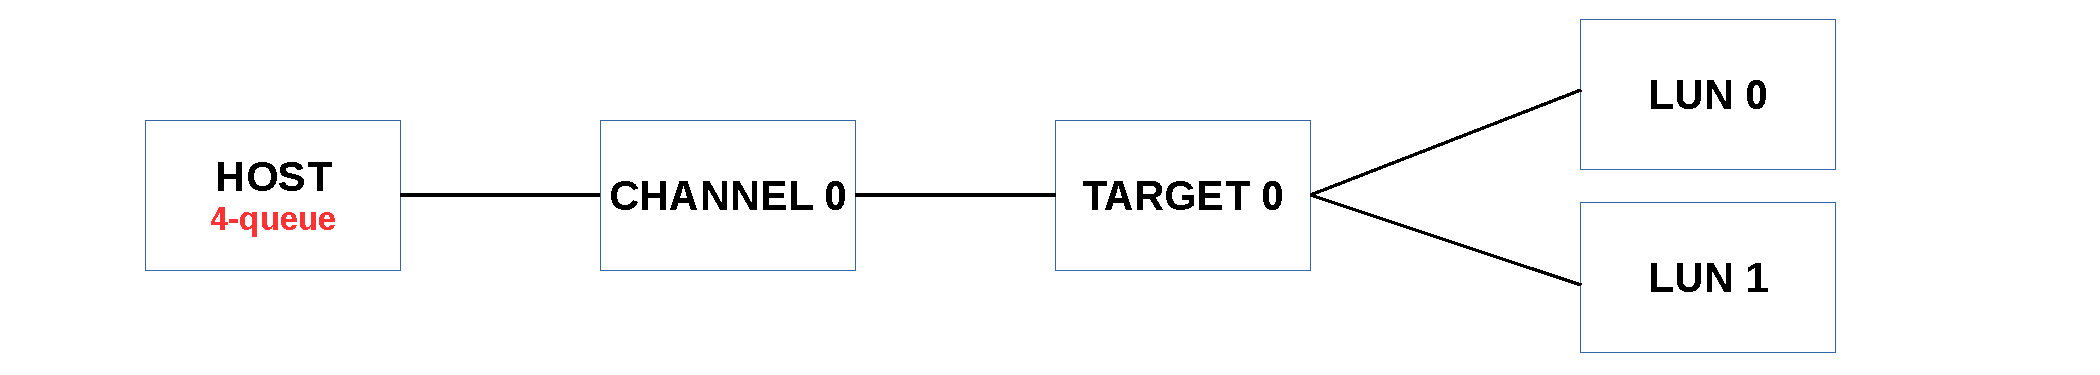
\includegraphics[width=1.0\linewidth]{figures/virtscsi.pdf}
\end{figure}
\begin{block}{}
[    0.604610] scsi host0: \textbf{\textcolor{blue}{Virtio SCSI HBA}}

[    0.606220] scsi \textcolor{red}{0:0:0:0}: Direct-Access     QEMU     QEMU HARDDISK    2.5+ PQ: 0 ANSI: 5

[    0.607168] scsi \textcolor{red}{0:0:0:1}: Direct-Access     QEMU     QEMU HARDDISK    2.5+ PQ: 0 ANSI: 5

[    0.617180] sd \textcolor{red}{0:0:0:0}: Attached scsi generic sg0 type 0

[    0.618537] sd \textcolor{red}{0:0:0:1}: [sdb] Attached SCSI disk

[    0.619014] sd \textcolor{red}{0:0:0:1}: Attached scsi generic sg1 type 0

[    0.625877] sd \textcolor{red}{0:0:0:0}: [sda] Attached SCSI disk
\end{block}
\end{frame}

%------------------------------------------------

\section{SCSI: virtio\_scsi 3/3}
\begin{frame}
\frametitle{SCSI: virtio\_scsi 3/3}
\begin{block}{}
\# ls /sys/block/sda/mq \\
\textcolor{red}{0  1  2  3}\\
\# ls /sys/block/sdb/mq \\
\textcolor{red}{0  1  2  3}\\
\end{block}
\begin{block}{}
\# cat /proc/interrupts $|$ grep virtio \\
\textcolor{red}{ 24: \ \ \ \ \ \ \ \ \ 0 \ \ \ \ \ \ \ \ \ \ 0 \ \ \ \ \ \ \ \ \ 0 \ \ \ \ \ \ \ 0   PCI-MSI 65536-edge \ \ \ \ virtio0-config} \\
\textcolor{red}{ 25: \ \ \ \ \ \ \ \ \ 0 \ \ \ \ \ \ \ \ \ \ 0 \ \ \ \ \ \ \ \ \ 0 \ \ \ \ \ \ \ 0   PCI-MSI 65537-edge \ \ \ \ virtio0-control} \\
\textcolor{red}{ 26: \ \ \ \ \ \ \ \ \ 0 \ \ \ \ \ \ \ \ \ \ 0 \ \ \ \ \ \ \ \ \ 0 \ \ \ \ \ \ \ 0   PCI-MSI 65538-edge \ \ \ \ virtio0-event} \\
\textcolor{red}{ 27: \ \ \ \ \ \ 1171 \ \ \ \ \ \ \ \ \ 0 \ \ \ \ \ \ \ \ \ 0 \ \ \ \ \ \ 0   PCI-MSI 65539-edge \ \ \ \ \textbf{\textcolor{blue}{virtio0-request}}} \\
\textcolor{red}{ 28: \ \ \ \ \ \ \ \ \ 0 \ \ \ \ \ \ 1180 \ \ \ \ \ \ \ \ \ 0 \ \ \ \ \ \ 0  PCI-MSI 65540-edge \ \ \ \ \textbf{\textcolor{blue}{virtio0-request}}} \\
\textcolor{red}{ 29: \ \ \ \ \ \ \ \ \ 0 \ \ \ \ \ \ \ \ \ \ 0 \ \ \ \ \ \ \ 831 \ \ \ \ \ \ 0   PCI-MSI 65541-edge \ \ \ \ \textbf{\textcolor{blue}{virtio0-request}}} \\
\textcolor{red}{ 30: \ \ \ \ \ \ \ \ \ 0 \ \ \ \ \ \ \ \ \ \ 0 \ \ \ \ \ \ \ \ \ \ 0 \ \ \ 1636   PCI-MSI 65542-edge \ \ \ \ \textbf{\textcolor{blue}{virtio0-request}}}
\end{block}
\end{frame}

%------------------------------------------------

\section{NVMe 1/2}
\begin{frame}
\frametitle{NVMe 1/2}
{\LARGE NVMe device with 8 hardware queues}
\begin{itemize}
\item {\large Customize \textbf{\textcolor{blue}{num\_queues}} to test how NVMe driver works with different \#queues}
\end{itemize}
\begin{block}{}

\# qemu-system-x86\_64 -machine accel=kvm -vnc :0 -smp 4 -m 4096M \textbackslash

-net nic -net user,hostfwd=tcp::5022-:22 \textbackslash

-kernel /home/user/linux/arch/x86\_64/boot/bzImage \textbackslash
	
-append "root=/dev/sda1 init=/sbin/init text" \textbackslash

-hda /home/user/img/boot.qcow2 \textbackslash

\textcolor{red}{-device \textbf{\textcolor{blue}{nvme}},drive=nvme0,serial=deadbeaf1,\textbf{\textcolor{blue}{num\_queues}}=8} \textbackslash

\textcolor{red}{-drive file=/home/user/img/disk.qcow2,if=none,id=nvme0}

\end{block}
\end{frame}

%------------------------------------------------

\section{NVMe 2/2}
\begin{frame}
\frametitle{NVMe 2/2}
\begin{block}{}
[    0.576209] nvme nvme0: pci function 0000:00:04.0

[    0.620458] nvme nvme0: \textbf{\textcolor{red}{4/0/0 default/read/poll queues}}
\end{block}
\begin{block}{}
\# ls /dev/nvme0

\textcolor{red}{nvme0 \ \ nvme0n1}
\end{block}
\begin{block}{}
\# cat /proc/interrupts $|$ grep nvme \\
\textcolor{red}{ 24: \ \ \ \ \ \ 11 \ \ \ \ \ \ 0 \ \ \ \ \ \ \ \ \ \ 0 \ \ \ 0 \ \ PCI-MSI 65536-edge \ \ \ \ nvme0q0} \\
\textcolor{red}{ 25: \ \ \ \ \ \ 40 \ \ \ \ \ \ 0 \ \ \ \ \ \ \ \ \ \ 0 \ \ \ 0 \ \ PCI-MSI 65537-edge \ \ \ \ \textbf{\textcolor{blue}{nvme0q1}}} \\
\textcolor{red}{ 26: \ \ \ \ \ \ \ 0 \ \ \ \ \ \ 0 \ \ \ \ \ \ \ \ \ \ 0 \ \ \ 0 \ \ PCI-MSI 65538-edge \ \ \ \ \textbf{\textcolor{blue}{nvme0q2}}} \\
\textcolor{red}{ 27: \ \ \ \ \ \ \ 0 \ \ \ \ \ \ 0 \ \ \ \ \ \ \ \ \ 41 \ \ \ 0 \ \ PCI-MSI 65539-edge \ \ \ \ \textbf{\textcolor{blue}{nvme0q3}}} \\
\textcolor{red}{ 28: \ \ \ \ \ \ \ 0 \ \ \ \ \ \ 0 \ \ \ \ \ \ \ \ \ \ 0 \ \ \ 0 \ \ PCI-MSI 65540-edge \ \ \ \ \textbf{\textcolor{blue}{nvme0q4}}}
\end{block}
\end{frame}

%------------------------------------------------

\section{NVDIMM 1/2}
\begin{frame}
\frametitle{NVDIMM 1/2}
{\LARGE NVDIMM: Non-Volatile Dual In-line Memory Module}
\begin{itemize}
\item {\large \textbf{\textcolor{olive}{pmem}} and \textbf{\textcolor{olive}{blk}} types}
\item {\large QEMU supports only \textbf{\textcolor{olive}{pmem}} type}
\end{itemize}
\begin{block}{}

\# qemu-system-x86\_64 -vnc :0 -smp 4 \textbackslash

-machine pc,\textbf{\textcolor{blue}{nvdimm}},accel=kvm \textbackslash

\textcolor{red}{-m 2G,maxmem=10G,slots=4} \textbackslash

\textcolor{red}{-object memory-backend-file,share,id=mem1,mem-path=nvdimm.img,size=16G} \textbackslash

\textcolor{red}{-device \textbf{\textcolor{blue}{nvdimm}},memdev=mem1,id=nvdimm1} \textbackslash

-net nic -net user,hostfwd=tcp::5022-:22 \textbackslash

-hda /home/user/img/boot.qcow2 \textbackslash

-kernel /home/user/linux/arch/x86\_64/boot/bzImage \textbackslash

-append "root=/dev/sda1 init=/sbin/init text"

\end{block}
\end{frame}

%------------------------------------------------

\section{NVDIMM 2/2}
\begin{frame}
\frametitle{NVDIMM 2/2}
{\LARGE Install utility library for managing the libnvdimm}
\begin{itemize}
\item {\large sudo apt-get install \textbf{\textcolor{olive}{libndctl ndctl}}}
\item {\large https://github.com/pmem/ndctl}
\end{itemize}
\begin{columns}[c]
\column{.45\textwidth}
\begin{block}{}
{ \small
CONFIG\_BLK\_DEV\_RAM\_DAX=y \\
CONFIG\_FS\_DAX=y \\
CONFIG\_X86\_PMEM\_LEGACY=y \\
CONFIG\_LIBNVDIMM=y \\
CONFIG\_BLK\_DEV\_PMEM=m \\
CONFIG\_ARCH\_HAS\_PMEM\_API=y \\
CONFIG\_TRANSPARENT\_HUGEPAGE=y \\
CONFIG\_MEMORY\_HOTPLUG=y \\
CONFIG\_MEMORY\_HOTREMOVE=y \\
CONFIG\_ZONE\_DEVICE=y \\
CONFIG\_FS\_DAX\_PMD=y  \\
\textcolor{red}{CONFIG\_ACPI\_NFIT=y}
}
\end{block}
\column{.45\textwidth}
\begin{block}{}
\# \textbf{\textcolor{blue}{ndctl list}}

{
\textcolor{red}{\ \  "dev":"\textbf{\textcolor{blue}{namespace0.0}}",}
	  
\textcolor{red}{\ \  "mode":"raw",}
  
\textcolor{red}{\ \  "size":17179869184,}
  
\textcolor{red}{\ \  "sector\_size":512,}
  
\textcolor{red}{\ \  "blockdev":"\textbf{\textcolor{blue}{pmem0}}",}
  
\textcolor{red}{\ \  "numa\_noe":0}

}
\end{block}
\end{columns}
\end{frame}

%------------------------------------------------

\section{Virtio Block 1/2}
\begin{frame}
\frametitle{Virtio Block 1/2}
{\LARGE Virtio Block device with 4 hardware queues}

\begin{block}{}

\# qemu-system-x86\_64 -machine accel=kvm -vnc :0 -smp 4 -m 4096M \textbackslash

-net nic -net user,hostfwd=tcp::5022-:22 \textbackslash

-kernel /home/user/linux/arch/x86\_64/boot/bzImage \textbackslash
	
-append "root=/dev/sda1 init=/sbin/init text" \textbackslash

-hda /home/user/img/boot.qcow2 \textbackslash

\textcolor{red}{-device \textbf{\textcolor{blue}{virtio-blk-pci}},drive=drive0,id=virtblk0,\textbf{\textcolor{blue}{num-queues=4}}} \textbackslash

\textcolor{red}{-drive file=/home/user/img/disk.qcow2,if=none,id=drive0}

\end{block}
\end{frame}

%------------------------------------------------

\section{Virtio Block 2/2}
\begin{frame}
\frametitle{Virtio Block 2/2}
\begin{block}{}
\# ls /dev/vda \newline
\textcolor{red}{/dev/vda} \newline

\#ls /sys/block/vda/mq/ \newline
\textcolor{red}{0 1 2 3} \newline

\#cat /proc/interrupts $|$ grep virtio \newline
\textcolor{red}{\ 24:\ \ \ \ \ \ \ \ \ \ 0\ \ \ \ \ \ \ \ \ \ 0\ \ \ \ \ \ \ \ \ \ 0\ \ \ \ \ \ \ \ \ \ 0\ \ \ PCI-MSI 65536-edge\ \ \ \ \ \ virtio0-config} \newline
\textcolor{red}{\ 25:\ \ \ \ \ \ \ \ \ \ 1\ \ \ \ \ \ \ \ \ \ 0\ \ \ \ \ \ \ \ \ \ 0\ \ \ \ \ \ \ \ \ \ 0\ \ \ PCI-MSI 65537-edge\ \ \ \ \ \ \textbf{\textcolor{blue}{virtio0-req.0}}} \newline
\textcolor{red}{\ 26:\ \ \ \ \ \ \ \ \ \ 0\ \ \ \ \ \ \ \ \ 30\ \ \ \ \ \ \ \ \ \ 0\ \ \ \ \ \ \ \ \ \ 0\ \ \ PCI-MSI 65538-edge\ \ \ \ \ \ \textbf{\textcolor{blue}{virtio0-req.1}}} \newline
\textcolor{red}{\ 27:\ \ \ \ \ \ \ \ \ \ 0\ \ \ \ \ \ \ \ \ \ 0\ \ \ \ \ \ \ \ \ 33\ \ \ \ \ \ \ \ \ \ 0\ \ \ PCI-MSI 65539-edge\ \ \ \ \ \ \textbf{\textcolor{blue}{virtio0-req.2}}} \newline
\textcolor{red}{\ 28:\ \ \ \ \ \ \ \ \ \ 0\ \ \ \ \ \ \ \ \ \ 0\ \ \ \ \ \ \ \ \ \ 0\ \ \ \ \ \ \ \ \ \ 0\ \ \ PCI-MSI 65540-edge\ \ \ \ \ \ \textbf{\textcolor{blue}{virtio0-req.3}}}
\end{block}
\end{frame}

%------------------------------------------------

\section{QEMU Tap Bridge Helper Script}
\begin{frame}
\frametitle{QEMU Tap Bridge Helper Script}
\begin{itemize}
\item The script bridges \textbf{\textcolor{blue}{tap}} created by QEMU to \textcolor{red}{host bridge} (e.g., br0)
\item Used by QEMU \textbf{\textcolor{blue}{-netdev}} during VM creation
\end{itemize}
\begin{block}{}
\# cat /home/user/qemu-ifup \newline

\textcolor{red}{\#! /bin/sh} \newline
\textcolor{red}{\# Script to bring a network (tap) device for qemu up.} \newline

\textcolor{red}{br="br0"} \newline

\textcolor{red}{ifconfig \$1 up} \newline
\textcolor{red}{brctl addif \$br "\$1"} \newline

\textcolor{red}{exit}
\end{block}
\end{frame}

%------------------------------------------------

\section{Virtio Net 1/2}
\begin{frame}
\frametitle{Virtio Net 1/2}
\begin{itemize}
\item To create Virtio Net device with \textbf{\textcolor{blue}{4}} queues (consuming 9 vectors)
\item \textbf{\textcolor{blue}{qemu-ifup}} is from previous slide
\item The \textbf{\textcolor{blue}{\#vector}} should be configured correctly (\textcolor{red}{4(TX)+4(RX)+1(Conf)=9})
\end{itemize}
\begin{block}{}
\# qemu-system-x86\_64 -machine accel=kvm -vnc :0 -smp 4 -m 4096M \textbackslash

-kernel /home/user/linux/arch/x86\_64/boot/bzImage \textbackslash
	
-append "root=/dev/sda1 init=/sbin/init text" \textbackslash

-hda /home/user/img/boot.qcow2 \textbackslash

\textcolor{red}{-device \textbf{\textcolor{blue}{virtio-net-pci}},netdev=tapnet,\textbf{\textcolor{blue}{mq=true,vectors=9}}} \textbackslash

\textcolor{red}{-netdev \textbf{\textcolor{blue}{tap}},id=tapnet,ifname=tap0,}\textbackslash

\textcolor{red}{\ \ \ \ script=/home/user/\textbf{\textcolor{blue}{qemu-ifup}},downscript=no,\textbf{\textcolor{blue}{queues=4}},vhost=off}

\end{block}
\end{frame}

%------------------------------------------------

\section{Virtio Net 2/2}
\begin{frame}
\frametitle{Virtio Net 2/2}
\begin{block}{}

host\# ip addr $|$ grep tap0 \newline
\textcolor{red}{34: \textbf{\textcolor{blue}{tap0}}: $<$BROADCAST,MULTICAST,UP,LOWER\_UP$>$ mtu 1500 qdisc \textbf{\textcolor{blue}{mq}} master \textbf{\textcolor{blue}{br0}} state UNKNOWN group default qlen 1000} \newline

vm\# cat /proc/interrupts $|$ grep virtio \newline
\textcolor{red}{\ 24:\ \ \ \ \ \ \ \ \ \ 0\ \ \ \ \ \ \ \ \ \ 0\ \ \ \ \ \ \ \ \ \ 0\ \ \ \ \ \ \ \ \ \ 0\ \ \ PCI-MSI 49152-edge\ \ \ \ \ \ virtio0-config} \newline
\textcolor{red}{\ 25:\ \ \ \ \ \ \ \ \ 57\ \ \ \ \ \ \ \ \ \ 1\ \ \ \ \ \ \ \ \ \ 0\ \ \ \ \ \ \ \ \ \ 0\ \ \ PCI-MSI 49153-edge\ \ \ \ \ \ \textbf{\textcolor{blue}{virtio0-input.0}}} \newline
\textcolor{red}{\ 26:\ \ \ \ \ \ \ \ \ \ 0\ \ \ \ \ \ \ \ \ \ 0\ \ \ \ \ \ \ \ \ \ 1\ \ \ \ \ \ \ \ \ \ 0\ \ \ PCI-MSI 49154-edge\ \ \ \ \ \ \textbf{\textcolor{blue}{virtio0-output.0}}} \newline
\textcolor{red}{\ 27:\ \ \ \ \ \ \ \ \ \ 0\ \ \ \ \ \ \ \ 110\ \ \ \ \ \ \ \ \ \ 0\ \ \ \ \ \ \ \ \ \ 1\ \ \ PCI-MSI 49155-edge\ \ \ \ \ \ \textbf{\textcolor{blue}{virtio0-input.1}}} \newline
\textcolor{red}{\ 28:\ \ \ \ \ \ \ \ \ \ 1\ \ \ \ \ \ \ \ \ \ 0\ \ \ \ \ \ \ \ \ \ 0\ \ \ \ \ \ \ \ \ \ 0\ \ \ PCI-MSI 49156-edge\ \ \ \ \ \ \textbf{\textcolor{blue}{virtio0-output.1}}} \newline
\textcolor{red}{\ 29:\ \ \ \ \ \ \ \ \ \ 0\ \ \ \ \ \ \ \ \ \ 1\ \ \ \ \ \ \ \ 135\ \ \ \ \ \ \ \ \ \ 0\ \ \ PCI-MSI 49157-edge\ \ \ \ \ \ \textbf{\textcolor{blue}{virtio0-input.2}}} \newline
\textcolor{red}{\ 30:\ \ \ \ \ \ \ \ \ \ 0\ \ \ \ \ \ \ \ \ \ 0\ \ \ \ \ \ \ \ \ \ 1\ \ \ \ \ \ \ \ \ \ 0\ \ \ PCI-MSI 49158-edge\ \ \ \ \ \ \textbf{\textcolor{blue}{virtio0-output.2}}} \newline
\textcolor{red}{\ 31:\ \ \ \ \ \ \ \ \ \ 0\ \ \ \ \ \ \ \ \ \ 0\ \ \ \ \ \ \ \ \ \ 0\ \ \ \ \ \ \ \ \ 49\ \ \ PCI-MSI 49159-edge\ \ \ \ \ \ \textbf{\textcolor{blue}{virtio0-input.3}}} \newline
\textcolor{red}{\ 32:\ \ \ \ \ \ \ \ \ \ 0\ \ \ \ \ \ \ \ \ \ 0\ \ \ \ \ \ \ \ \ \ 0\ \ \ \ \ \ \ \ \ \ 0\ \ \ PCI-MSI 49160-edge\ \ \ \ \ \ \textbf{\textcolor{blue}{virtio0-output.3}}}
\end{block}
\end{frame}

%------------------------------------------------

\section{E1000e}
\begin{frame}
\frametitle{E1000e}
The \textcolor{red}{e1000e} can be substituted by:
\begin{itemize}
\item \textcolor{red}{rtl8139}(8139cp), \textcolor{red}{vmxnet3}(vmxnet3), \textcolor{red}{i82550}(e100), \textcolor{red}{e1000}(e1000)
\end{itemize}
\begin{block}{}

\# qemu-system-x86\_64 -machine accel=kvm -vnc :0 -smp 4 -m 4096M \textbackslash

-kernel /home/user/linux/arch/x86\_64/boot/bzImage \textbackslash
	
-append "root=/dev/sda1 init=/sbin/init text" \textbackslash

-hda /home/user/img/boot.qcow2 \textbackslash

\textcolor{red}{-device \textbf{\textcolor{blue}{e1000e}},netdev=tapnet} \textbackslash

\textcolor{red}{-netdev tap,id=tapnet,ifname=tap0,script=/home/user/\textbf{\textcolor{blue}{qemu-ifup}},downscript=no}

\end{block}
\begin{block}{}
vm\# ethtool -i enp0s3 $|$ grep driver \newline
\textcolor{red}{driver: e1000e}
\end{block}
\end{frame}

%------------------------------------------------

\section{PCI Bridge 1/3}
\begin{frame}
\frametitle{PCI Bridge 1/3}
{\LARGE Create 2 PCI-2-PCI bridge's secondary bus}
\begin{itemize}
\item The 1st secondary bus is with 1 E1000 NIC
\item The 2nd secondary bus is with 2 E1000 NIC
\end{itemize}
\begin{block}{}

\# qemu-system-x86\_64 -machine \textbf{\textcolor{blue}{pc}},accel=kvm -vnc :0 -smp 4 -m 4096M \textbackslash

-net nic -net user,hostfwd=tcp::5022-:22 \textbackslash

-kernel /home/user/linux/arch/x86\_64/boot/bzImage \textbackslash
	
-append "root=/dev/sda1 init=/sbin/init text" \textbackslash

-hda /home/user/img/boot.qcow2 \textbackslash

\textcolor{red}{-device \textbf{\textcolor{blue}{pci-bridge}},id=bridge0,chassis\_nr=1} \textbackslash

\textcolor{olive}{\ \ \ \ -device e1000,bus=bridge0,addr=0x3} \textbackslash

\textcolor{red}{-device \textbf{\textcolor{blue}{pci-bridge}},id=bridge1,chassis\_nr=2} \textbackslash

\textcolor{olive}{\ \ \ \ -device e1000,bus=bridge1,addr=0x3} \textbackslash

\textcolor{olive}{\ \ \ \ -device e1000,bus=bridge1,addr=0x4}

\end{block}
\end{frame}

%------------------------------------------------

\section{PCI Bridge 2/3}
\begin{frame}
\frametitle{PCI Bridge 2/3}
\begin{block}{}
00:00.0 Host bridge: Intel Corporation 440FX - 82441FX PMC [Natoma] (rev 02) \newline
00:01.0 ISA bridge: Intel Corporation 82371SB PIIX3 ISA [Natoma/Triton II] \newline
00:01.1 IDE interface: Intel Corporation 82371SB PIIX3 IDE [Natoma/Triton II] \newline
00:01.3 Bridge: Intel Corporation 82371AB/EB/MB PIIX4 ACPI (rev 03) \newline
00:02.0 VGA compatible controller: Device 1234:1111 (rev 02) \newline
00:03.0 Ethernet controller: Intel Corporation 82540EM Gigabit Ethernet Controller (rev 03) \newline
\textcolor{red}{00:04.0 PCI bridge: Red Hat, Inc. \textbf{\textcolor{blue}{QEMU PCI-PCI bridge}}} \newline
\textcolor{red}{00:05.0 PCI bridge: Red Hat, Inc. \textbf{\textcolor{blue}{QEMU PCI-PCI bridge}}} \newline
\textcolor{olive}{01:03.0 Ethernet controller: Intel Corporation 82540EM Gigabit Ethernet Controller (rev 03)} \newline
\textcolor{olive}{02:03.0 Ethernet controller: Intel Corporation 82540EM Gigabit Ethernet Controller (rev 03)} \newline
\textcolor{olive}{02:04.0 Ethernet controller: Intel Corporation 82540EM Gigabit Ethernet Controller (rev 03)}
\end{block}
\end{frame}

%------------------------------------------------

\section{PCI Bridge 3/3}
\begin{frame}
\frametitle{PCI Bridge 3/3}
\begin{figure}
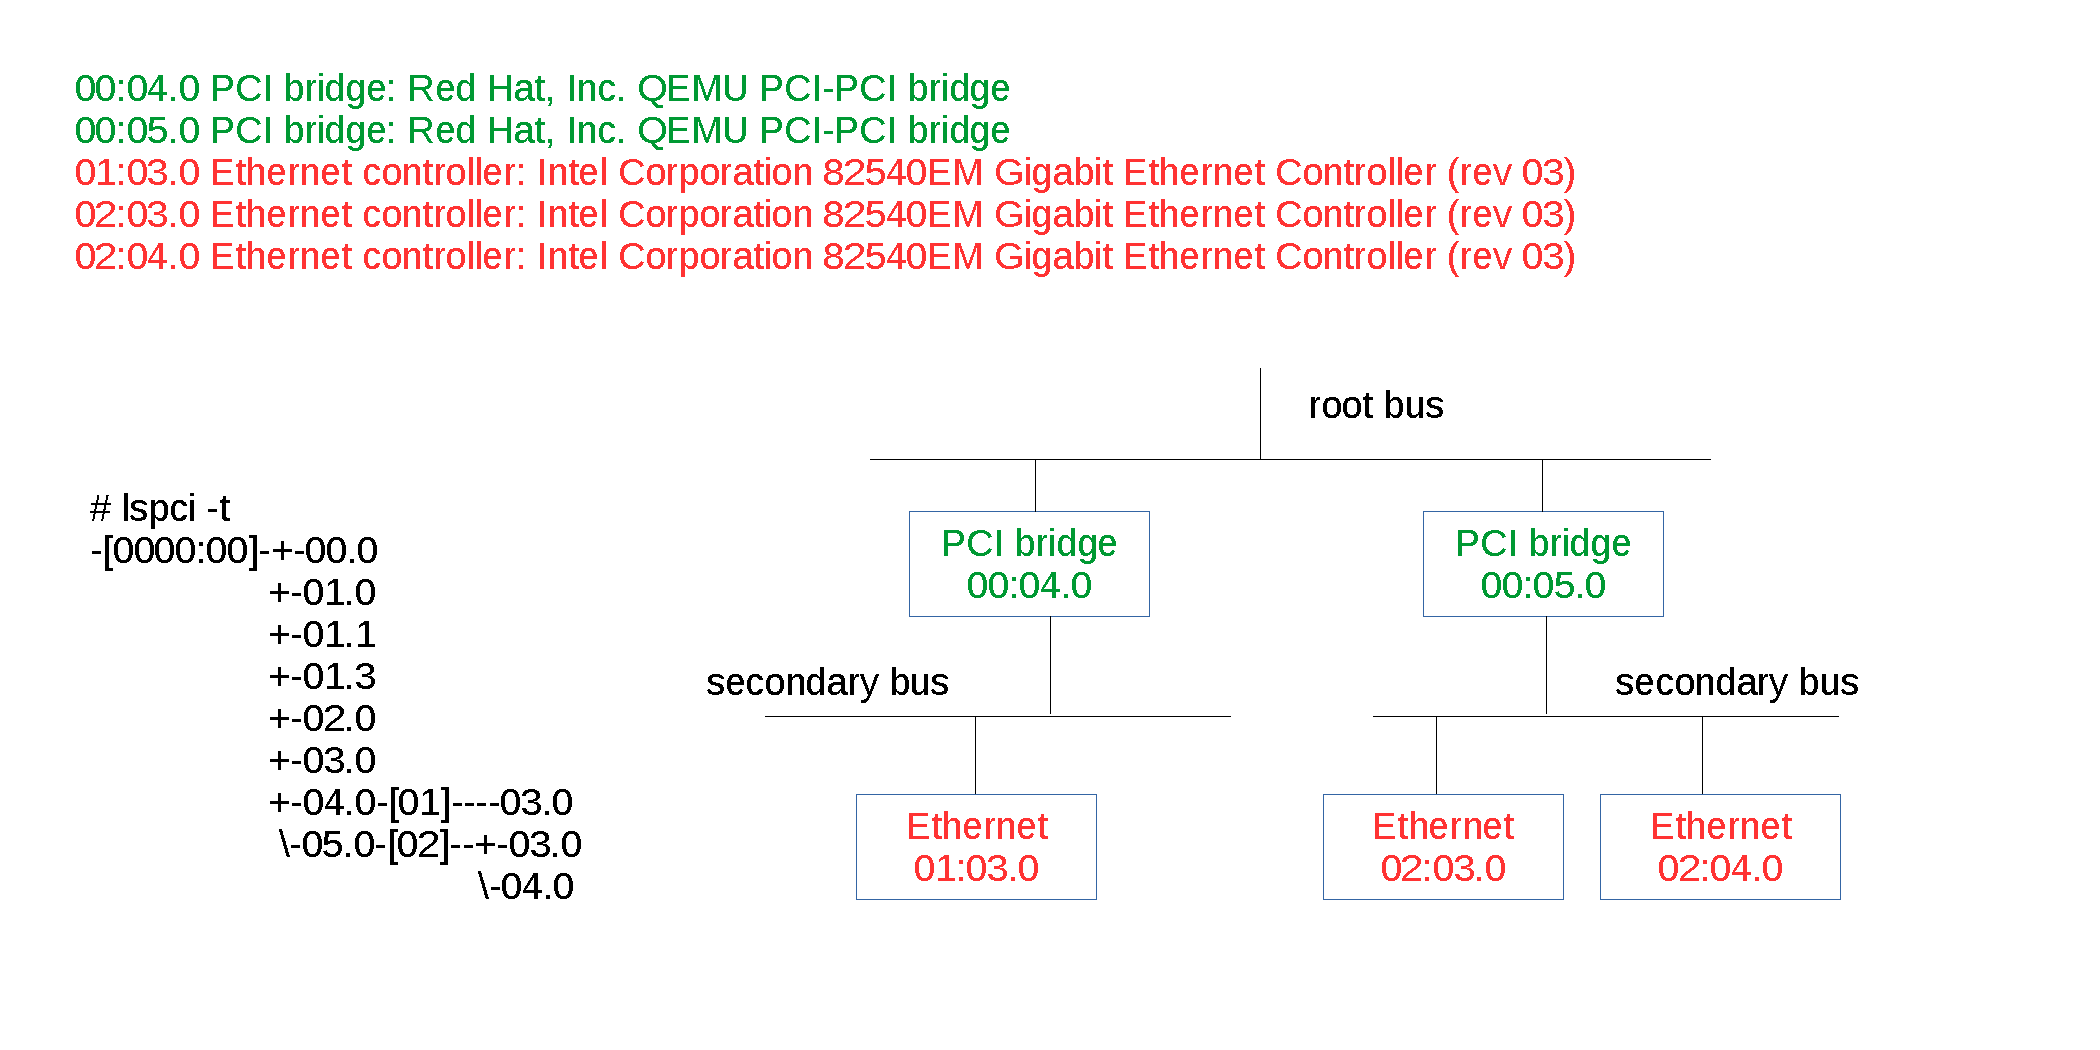
\includegraphics[width=1.0\linewidth]{figures/pci-secondary.pdf}
\end{figure}
\end{frame}

%------------------------------------------------

\section{PCI Root Bus 1/3}
\begin{frame}
\frametitle{PCI Root Bus 1/3}
{\LARGE Create 2 PCI Expander Bridge (PXB)'s primary bus}
\begin{itemize}
\item The 1st primary bus is with 1 E1000 NIC
\item The 2nd primary bus is with 2 E1000 NIC
\end{itemize}
\begin{block}{}

\# qemu-system-x86\_64 -machine \textbf{\textcolor{blue}{pc}},accel=kvm -vnc :0 -smp 4 -m 4096M \textbackslash

-net nic -net user,hostfwd=tcp::5022-:22 \textbackslash

-kernel /home/user/linux/arch/x86\_64/boot/bzImage \textbackslash
	
-append "root=/dev/sda1 init=/sbin/init text" \textbackslash

-hda /home/user/img/boot.qcow2 \textbackslash

\textcolor{red}{-device \textbf{\textcolor{blue}{pxb}},id=bridge1,bus=pci.0,bus\_nr=3} \textbackslash

\textcolor{olive}{\ \ \ \ -device e1000,bus=bridge1,addr=0x3} \textbackslash

\textcolor{red}{-device \textbf{\textcolor{blue}{pxb}},id=bridge2,bus=pci.0,bus\_nr=8} \textbackslash

\textcolor{olive}{\ \ \ \ -device e1000,bus=bridge2,addr=0x3} \textbackslash

\textcolor{olive}{\ \ \ \ -device e1000,bus=bridge2,addr=0x4}

\end{block}
\end{frame}

%------------------------------------------------

\section{PCI Root Bus 2/3}
\begin{frame}
\frametitle{PCI Root Bus 2/3}
\begin{block}{}
00:00.0 Host bridge: Intel Corporation 440FX - 82441FX PMC [Natoma] (rev 02) \newline
00:01.0 ISA bridge: Intel Corporation 82371SB PIIX3 ISA [Natoma/Triton II] \newline
00:01.1 IDE interface: Intel Corporation 82371SB PIIX3 IDE [Natoma/Triton II] \newline
00:01.3 Bridge: Intel Corporation 82371AB/EB/MB PIIX4 ACPI (rev 03) \newline
00:02.0 VGA compatible controller: Device 1234:1111 (rev 02) \newline
00:03.0 Ethernet controller: Intel Corporation 82540EM Gigabit Ethernet Controller (rev 03) \newline
\textcolor{red}{00:04.0 Host bridge: Red Hat, Inc. QEMU \textbf{\textcolor{blue}{PCI Expander bridge}}} \newline
\textcolor{red}{00:05.0 Host bridge: Red Hat, Inc. QEMU \textbf{\textcolor{blue}{PCI Expander bridge}}} \newline
\textcolor{red}{03:00.0 PCI bridge: Red Hat, Inc. QEMU \textbf{\textcolor{blue}{PCI-PCI bridge}}} \newline
\textcolor{olive}{04:03.0 Ethernet controller: Intel Corporation 82540EM Gigabit Ethernet Controller (rev 03)} \newline
\textcolor{red}{08:00.0 PCI bridge: Red Hat, Inc. QEMU \textbf{\textcolor{blue}{PCI-PCI bridge}}} \newline
\textcolor{olive}{09:03.0 Ethernet controller: Intel Corporation 82540EM Gigabit Ethernet Controller (rev 03)} \newline
\textcolor{olive}{09:04.0 Ethernet controller: Intel Corporation 82540EM Gigabit Ethernet Controller (rev 03)}
\end{block}
\end{frame}

%------------------------------------------------

\section{PCI Root Bus 3/3}
\begin{frame}
\frametitle{PCI Root Bus 3/3}
\begin{figure}
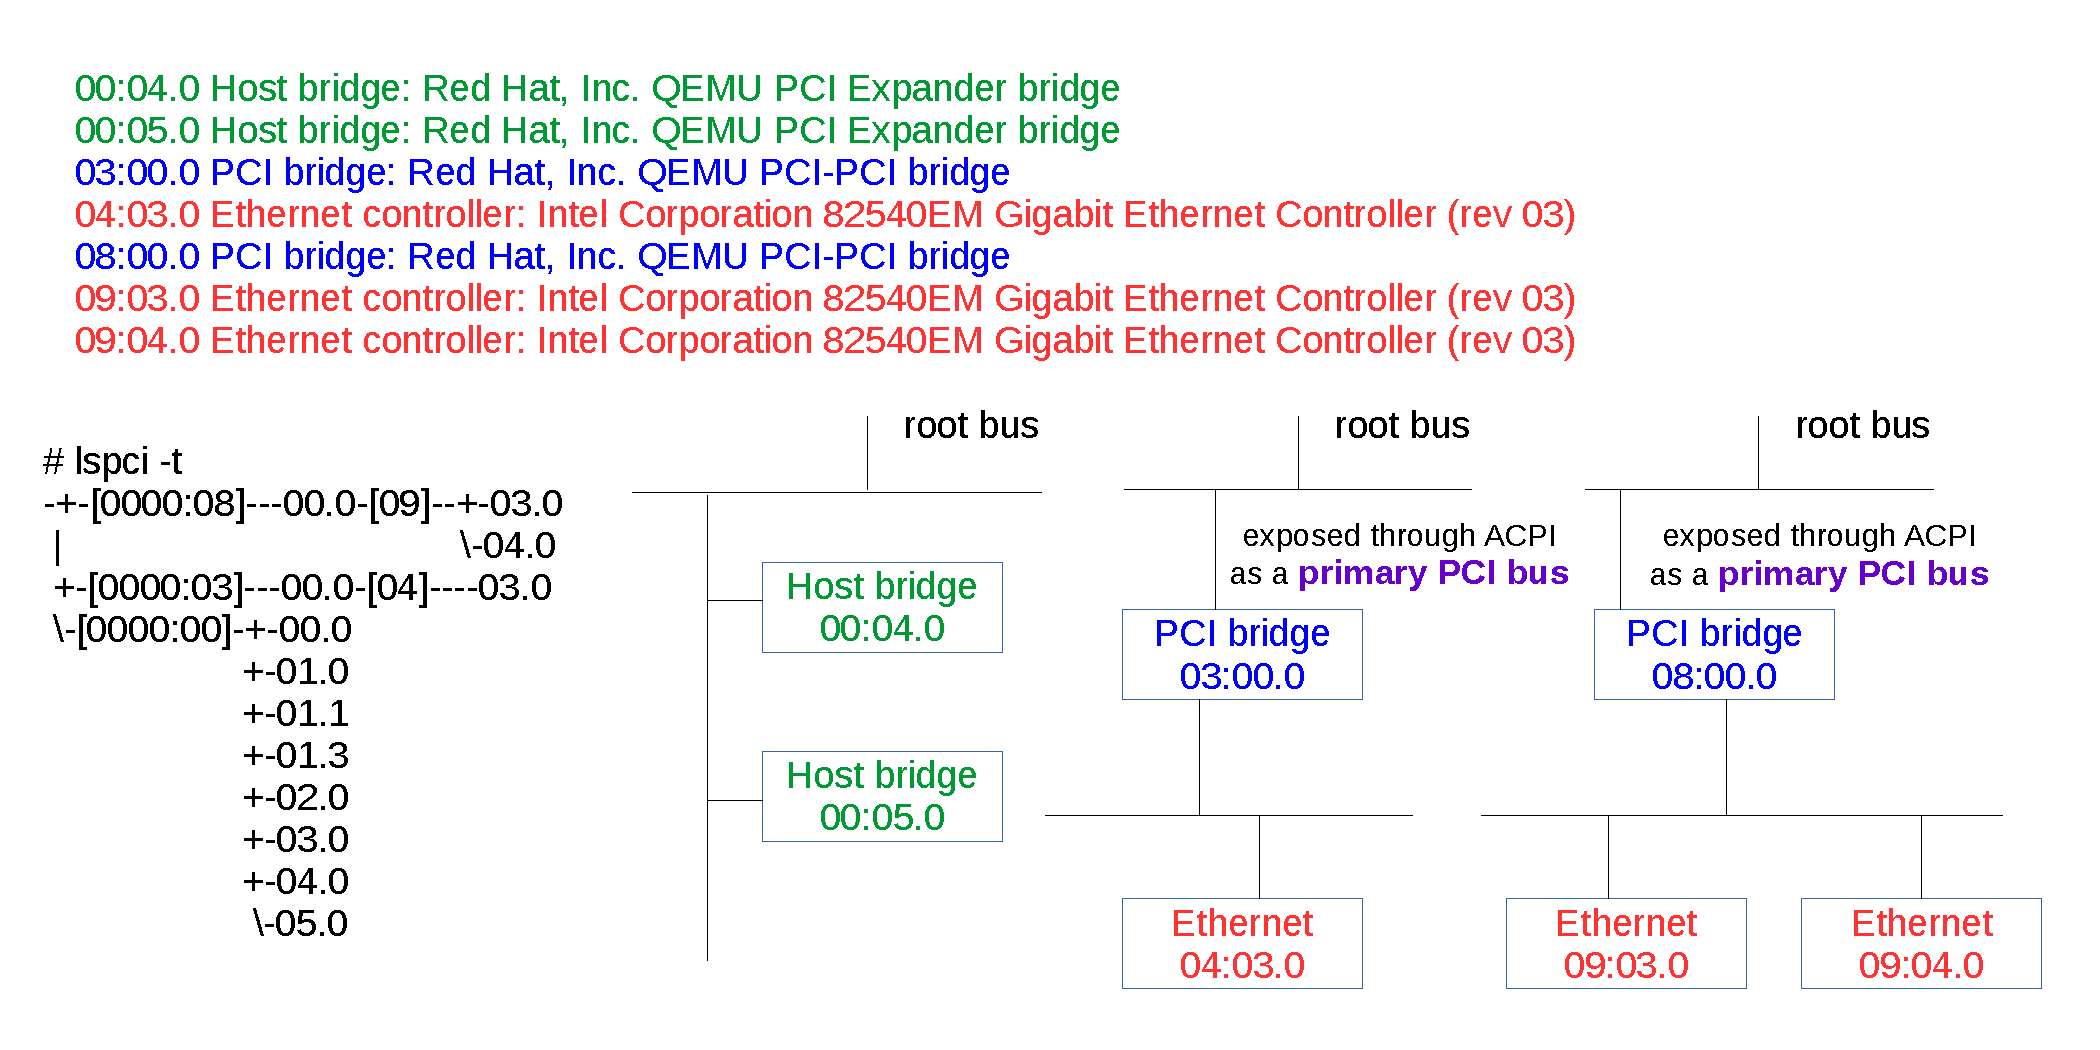
\includegraphics[width=1.0\linewidth]{figures/pci-primary.pdf}
\end{figure}
\end{frame}

%------------------------------------------------

\section{PCI Express Root Complex 1/3}
\begin{frame}
\frametitle{PCI Express Root Complex 1/3}
{\LARGE Create 2 extra PCI Express Root Complex}
\begin{itemize}
\item The 1st PCI Express Root Complex is with 2 E1000 NIC
\item The 2nd PCI Express Root Complex is with 1 E1000 NIC
\end{itemize}
\begin{block}{}
\small
\# qemu-system-x86\_64 -machine \textbf{\textcolor{blue}{q35}},accel=kvm -vnc :0 -smp 4 -m 4096M \textbackslash

-net nic -net user,hostfwd=tcp::5022-:22 \textbackslash

-kernel /home/user/linux/arch/x86\_64/boot/bzImage \textbackslash
	
-append "root=/dev/sda1 init=/sbin/init text" \textbackslash

-hda /home/user/img/boot.qcow2 \textbackslash

\textcolor{red}{-device \textbf{\textcolor{blue}{pxb-pcie}},id=pcie.1,bus\_nr=2,bus=pcie.0} \textbackslash

\textcolor{red}{\ \ \ \ -device \textbf{\textcolor{blue}{ioh3420}},id=pcie\_pci\_bridge1,bus=pcie.1,chassis=1} \textbackslash

\textcolor{olive}{\ \ \ \ \ \ \ \ -device e1000e,bus=pcie\_pci\_bridge1} \textbackslash

\textcolor{red}{\ \ \ \ -device \textbf{\textcolor{blue}{ioh3420}},id=pcie\_pci\_bridge2,bus=pcie.1,chassis=2} \textbackslash

\textcolor{olive}{\ \ \ \ \ \ \ \ -device e1000e,bus=pcie\_pci\_bridge2} \textbackslash

\textcolor{red}{-device \textbf{\textcolor{blue}{pxb-pcie}},id=pcie.2,bus\_nr=8,bus=pcie.0} \textbackslash

\textcolor{red}{\ \ \ \ -device \textbf{\textcolor{blue}{ioh3420}},id=pcie\_pci\_bridge3,bus=pcie.2,chassis=3} \textbackslash

\textcolor{olive}{\ \ \ \ \ \ \ \ -device e1000e,bus=pcie\_pci\_bridge3}

\end{block}
\end{frame}

%------------------------------------------------

\section{PCI Express Root Complex 2/3}
\begin{frame}
\frametitle{PCI Express Root Complex 2/3}
\begin{block}{}
\small
00:00.0 Host bridge: Intel Corporation 82G33/G31/P35/P31 Express DRAM Controller \newline
00:01.0 VGA compatible controller: Device 1234:1111 (rev 02) \newline
00:02.0 Ethernet controller: Intel Corporation 82574L Gigabit Network Connection \newline
\textcolor{red}{00:03.0 Host bridge: Red Hat, Inc. QEMU \textbf{\textcolor{blue}{PCIe Expander bridge}}} \newline
\textcolor{red}{00:04.0 Host bridge: Red Hat, Inc. QEMU \textbf{\textcolor{blue}{PCIe Expander bridge}}} \newline
00:1f.0 ISA bridge: Intel Corporation 82801IB (ICH9) LPC Interface Controller (rev 02) \newline
00:1f.2 SATA controller: Intel Corporation 82801IR/IO/IH (ICH9R/DO/DH) 6 port SATA Controller [AHCI mode] (rev 02) \newline
00:1f.3 SMBus: Intel Corporation 82801I (ICH9 Family) SMBus Controller (rev 02) \newline
\textcolor{red}{02:00.0 PCI bridge: Intel Corporation 7500/5520/5500/X58 \textbf{\textcolor{blue}{I/O Hub PCI Express Root Port}} 0}  \newline
\textcolor{red}{02:01.0 PCI bridge: Intel Corporation 7500/5520/5500/X58 \textbf{\textcolor{blue}{I/O Hub PCI Express Root Port}} 0}  \newline
\textcolor{olive}{03:00.0 Ethernet controller: Intel Corporation 82574L Gigabit Network Connection} \newline
\textcolor{olive}{04:00.0 Ethernet controller: Intel Corporation 82574L Gigabit Network Connection} \newline
\textcolor{red}{08:00.0 PCI bridge: Intel Corporation 7500/5520/5500/X58 \textbf{\textcolor{blue}{I/O Hub PCI Express Root Port}} 0}  \newline
\textcolor{olive}{09:00.0 Ethernet controller: Intel Corporation 82574L Gigabit Network Connection}
\end{block}
\end{frame}

%------------------------------------------------

\section{PCI Express Root Complex 3/3}
\begin{frame}
\frametitle{PCI Express Root Complex 3/3}
\begin{figure}
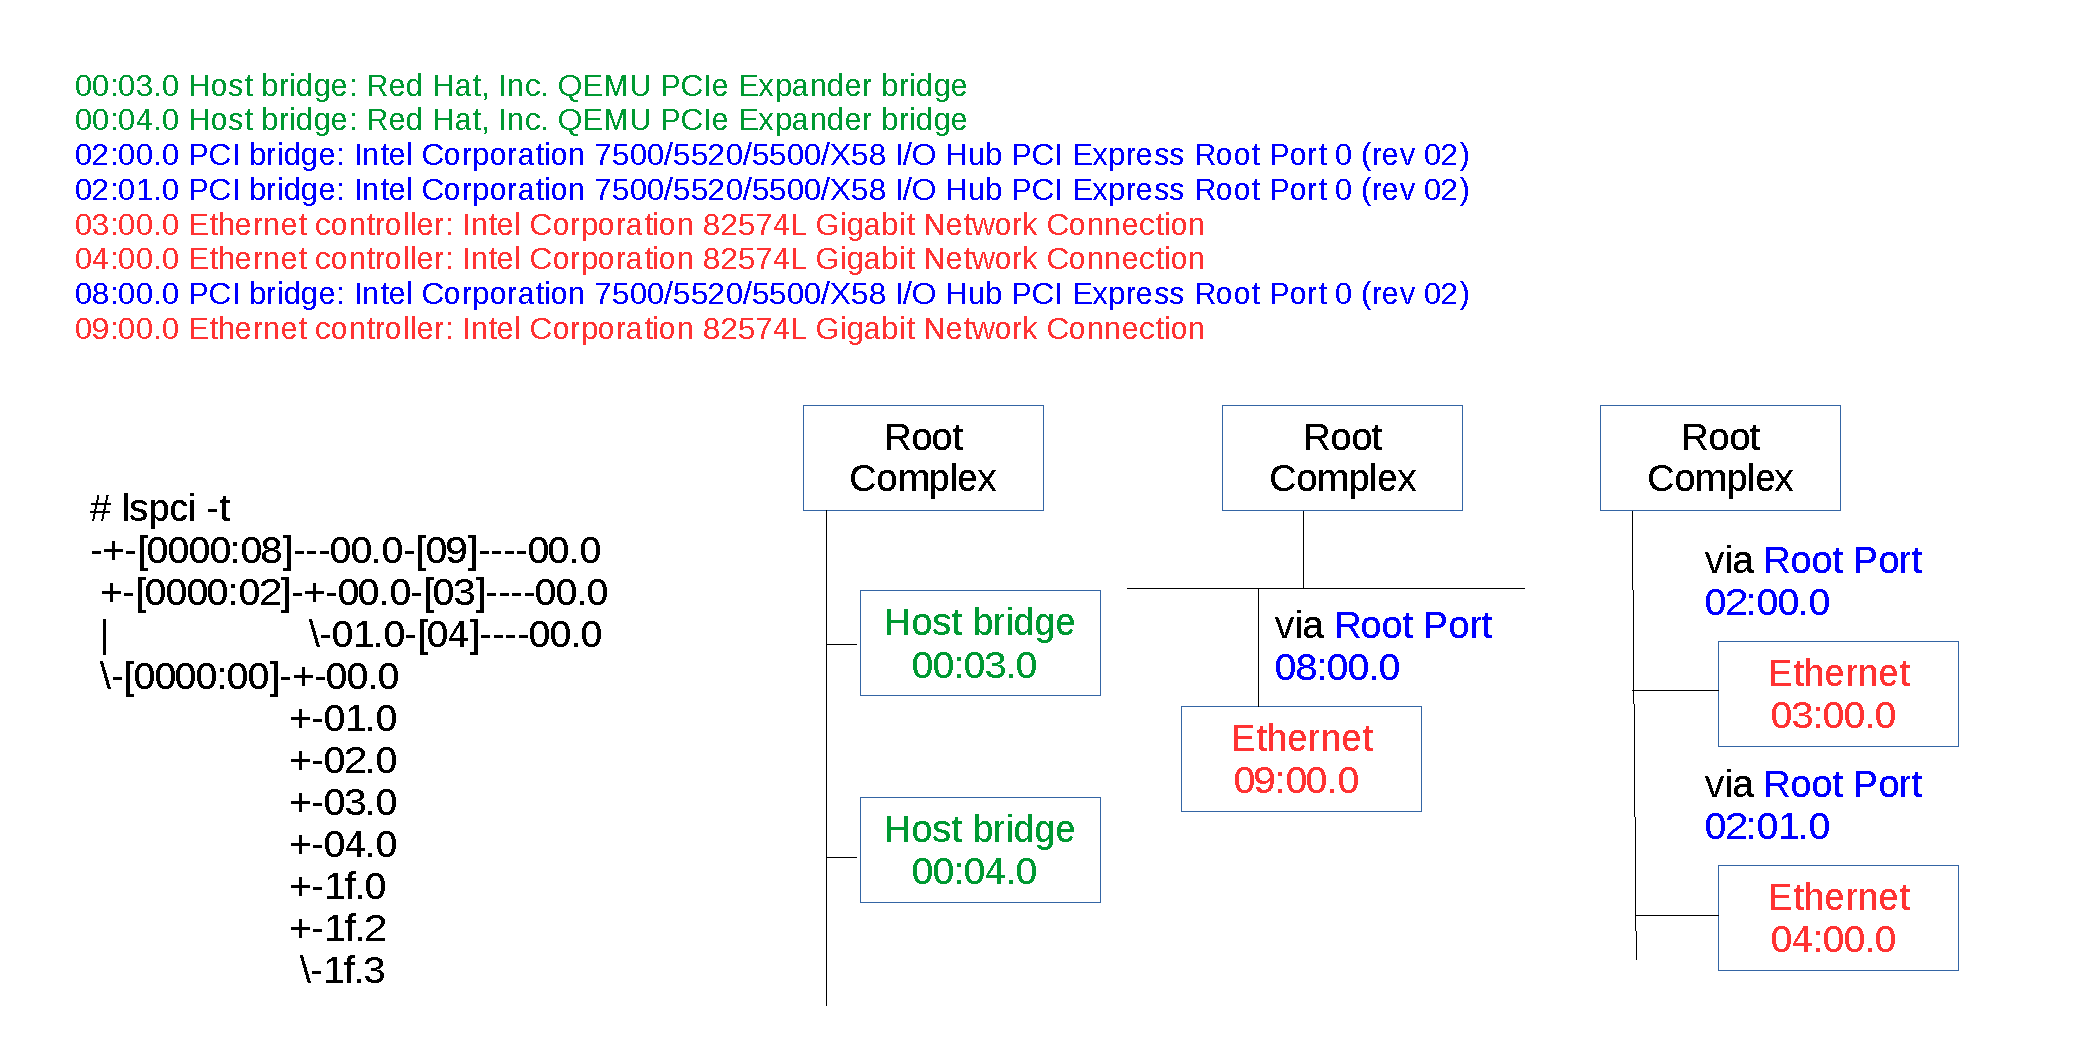
\includegraphics[width=1.0\linewidth]{figures/root-complex.pdf}
\end{figure}
\end{frame}

%------------------------------------------------

\section{PCI Express Switches 1/3}
\begin{frame}
\frametitle{PCI Express Switches 1/3}
{\LARGE Create 1 PCI Express Switch}
\begin{itemize}
\item There is 1 Upstream Port connecting to 2 Downstream Ports
\item Each Downstream Port is connected to 1 E1000e NIC
\end{itemize}
\begin{block}{}

\# qemu-system-x86\_64 -machine \textbf{\textcolor{blue}{q35}},accel=kvm -vnc :0 -smp 4 -m 4096M \textbackslash

-net nic -net user,hostfwd=tcp::5022-:22 \textbackslash

-kernel /home/user/linux/arch/x86\_64/boot/bzImage \textbackslash
	
-append "root=/dev/sda1 init=/sbin/init text" \textbackslash

-hda /home/user/img/boot.qcow2 \textbackslash

\textcolor{red}{-device \textbf{\textcolor{blue}{ioh3420}},id=root\_port1,bus=pcie.0} \textbackslash

\textcolor{red}{\ \ \ \ -device \textbf{\textcolor{blue}{x3130-upstream}},id=upstream1,bus=root\_port1} \textbackslash

\textcolor{red}{\ \ \ \ \ \ \ \ -device \textbf{\textcolor{blue}{xio3130-downstream}},id=downstream1,bus=upstream1,chassis=9} \textbackslash

\textcolor{olive}{\ \ \ \ \ \ \ \ \ \ \ \ -device e1000e,bus=downstream1} \textbackslash

\textcolor{red}{\ \ \ \ \ \ \ \ -device \textbf{\textcolor{blue}{xio3130-downstream}},id=downstream2,bus=upstream1,chassis=10} \textbackslash

\textcolor{olive}{\ \ \ \ \ \ \ \ \ \ \ \ -device e1000e,bus=downstream2}

\end{block}
\end{frame}

%------------------------------------------------

\section{PCI Express Switches 2/3}
\begin{frame}
\frametitle{PCI Express Switches 2/3}
\begin{block}{}
\small
00:00.0 Host bridge: Intel Corporation 82G33/G31/P35/P31 Express DRAM Controller \newline
00:01.0 VGA compatible controller: Device 1234:1111 (rev 02) \newline
00:02.0 Ethernet controller: Intel Corporation 82574L Gigabit Network Connection \newline
\textcolor{red}{00:03.0 PCI bridge: Intel Corporation 7500/5520/5500/X58 \textbf{\textcolor{blue}{I/O Hub PCI Express Root Port}} 0} \newline
00:1f.0 ISA bridge: Intel Corporation 82801IB (ICH9) LPC Interface Controller (rev 02) \newline
00:1f.2 SATA controller: Intel Corporation 82801IR/IO/IH (ICH9R/DO/DH) 6 port SATA Controller [AHCI mode] (rev 02) \newline
00:1f.3 SMBus: Intel Corporation 82801I (ICH9 Family) SMBus Controller (rev 02) \newline
\textcolor{red}{01:00.0 PCI bridge: Texas Instruments XIO3130 \textbf{\textcolor{blue}{PCI Express Switch (Upstream)}} (rev 02)} \newline
\textcolor{red}{02:00.0 PCI bridge: Texas Instruments XIO3130 \textbf{\textcolor{blue}{PCI Express Switch (Downstream)}} (rev 01)} \newline
\textcolor{red}{02:01.0 PCI bridge: Texas Instruments XIO3130 \textbf{\textcolor{blue}{PCI Express Switch (Downstream)}} (rev 01)} \newline
\textcolor{olive}{03:00.0 Ethernet controller: Intel Corporation 82574L Gigabit Network Connection} \newline
\textcolor{olive}{04:00.0 Ethernet controller: Intel Corporation 82574L Gigabit Network Connection}
\end{block}
\end{frame}

%------------------------------------------------

\section{PCI Express Switches 3/3}
\begin{frame}
\frametitle{PCI Express Switches 3/3}
\begin{figure}
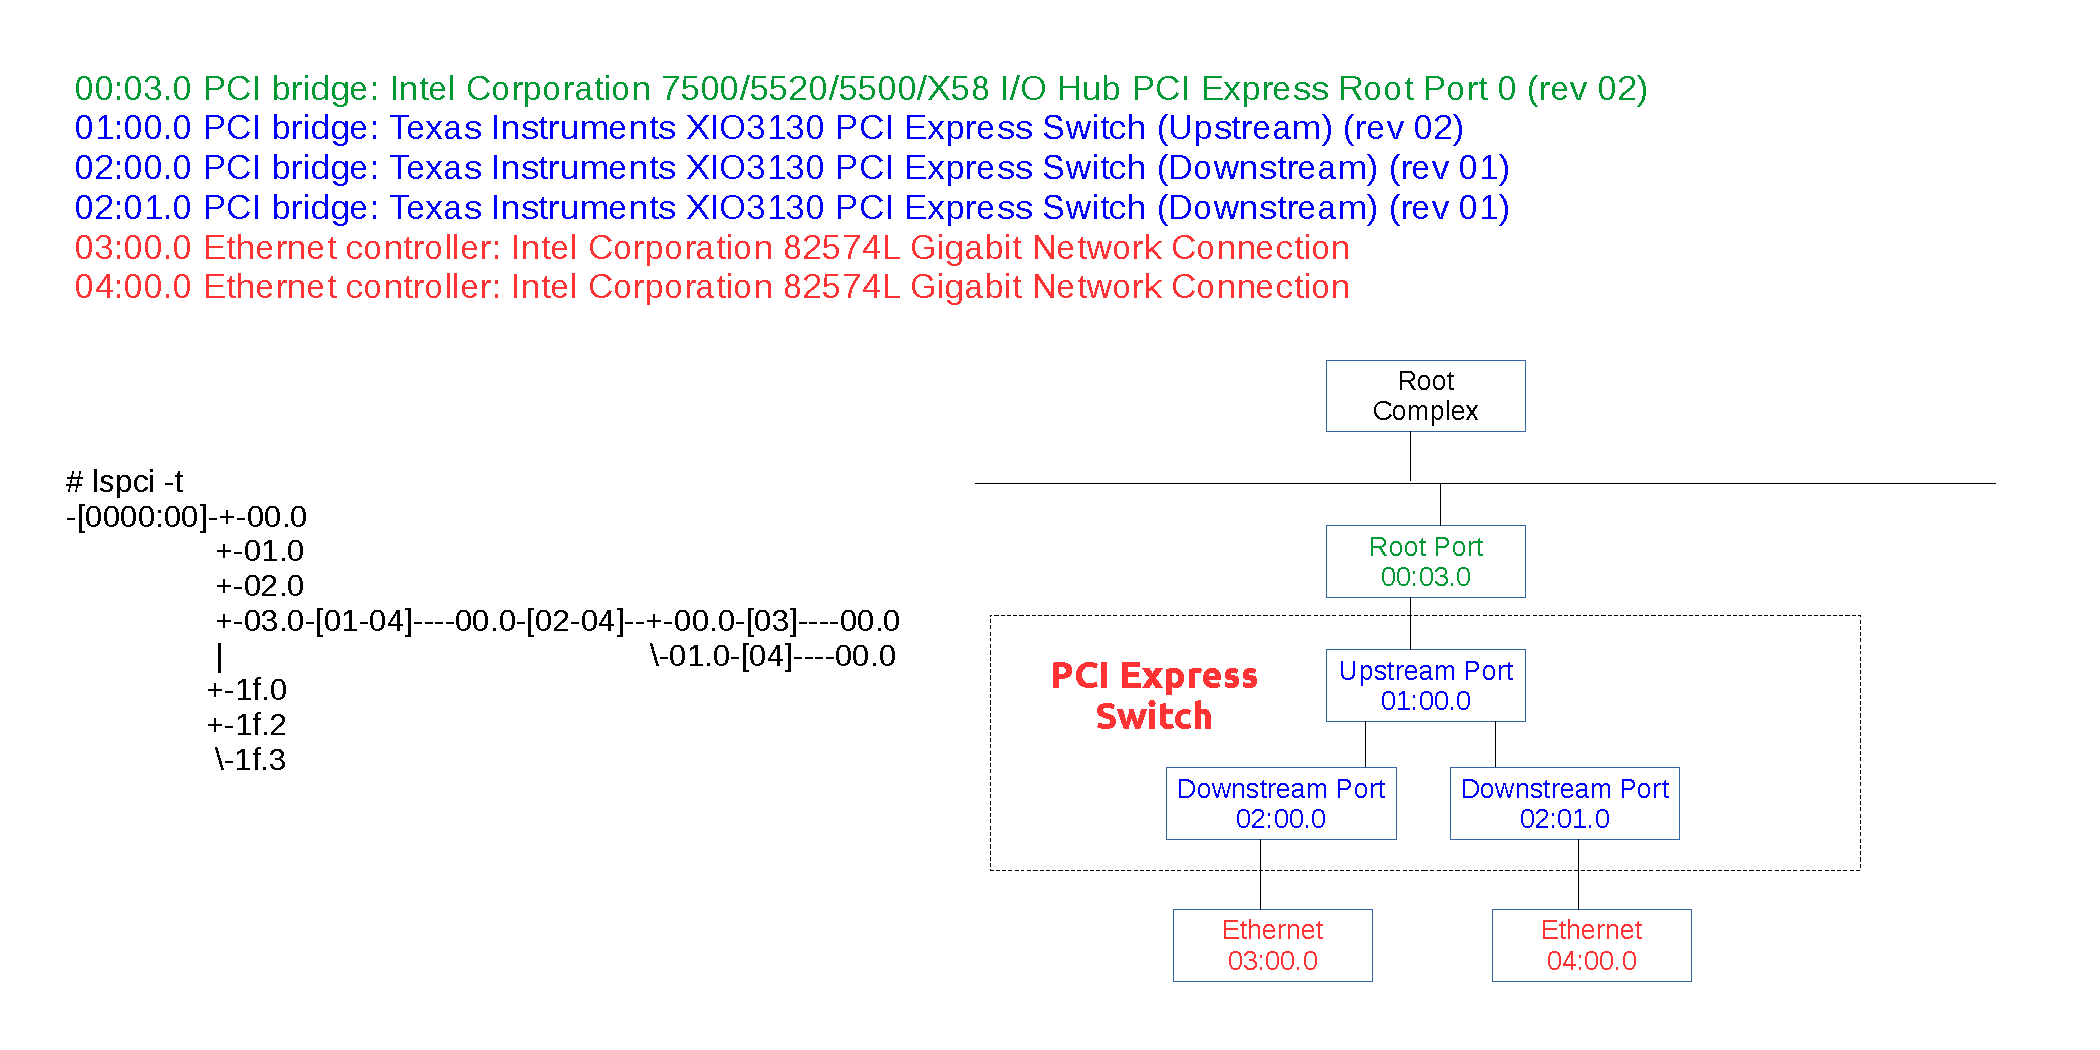
\includegraphics[width=1.0\linewidth]{figures/pcie-switch.pdf}
\end{figure}
\end{frame}

%------------------------------------------------

\section{IOMMU 1/2}
\begin{frame}
\frametitle{IOMMU 1/2}
{\LARGE Intel VT-d with Interrupt Remapping (IR) enabled}
\begin{itemize}
\item {\large Only \textbf{\textcolor{blue}{q35}} machine supports virtual IOMMU}
\item {\large \textbf{\textcolor{blue}{intel\_iommu=on}} should be added to kernel cmdline}
\end{itemize}
\begin{block}{}

\# qemu-system-x86\_64 -vnc :0 -smp 4 -m 4096M \textbackslash

\textcolor{red}{-machine \textbf{\textcolor{blue}{q35}},accel=kvm,kernel-irqchip=split} \textbackslash

-net nic -net user,hostfwd=tcp::5022-:22 \textbackslash

-kernel /home/user/linux/arch/x86\_64/boot/bzImage \textbackslash
	
-append "root=/dev/sda1 init=/sbin/init text \textbf{\textcolor{blue}{intel\_iommu=on}}" \textbackslash

-hda /home/user/img/boot.qcow2 \textbackslash

-device nvme,drive=nvme0,serial=deadbeaf1,num\_queues=8 \textbackslash

-drive file=/home/user/img/disk.qcow2,if=none,id=nvme0 \textbackslash

\textcolor{red}{-device \textbf{\textcolor{blue}{intel-iommu}},intremap=on}

\end{block}
\end{frame}

%------------------------------------------------

\section{IOMMU 2/2}
\begin{frame}
\frametitle{IOMMU 2/2}
\begin{block}{}
{\Large \# dmesg $|$ egrep "IOMMU$|$iommu"} \newline

\textcolor{red}{[    0.000000] DMAR: \textbf{\textcolor{blue}{IOMMU enabled}}} \newline
\textcolor{red}{[    0.003000] DMAR-IR: IOAPIC id 0 under DRHD base  0xfed90000 IOMMU 0} \newline
\textcolor{red}{[    0.477614] pci 0000:00:00.0: Adding to \textbf{\textcolor{blue}{iommu group}} 0} \newline
\textcolor{red}{[    0.478078] pci 0000:00:01.0: Adding to \textbf{\textcolor{blue}{iommu group}} 1} \newline
\textcolor{red}{[    0.478517] pci 0000:00:02.0: Adding to \textbf{\textcolor{blue}{iommu group}} 2} \newline
\textcolor{red}{[    0.478963] pci 0000:00:03.0: Adding to \textbf{\textcolor{blue}{iommu group}} 3} \newline
\textcolor{red}{[    0.479421] pci 0000:00:1f.0: Adding to \textbf{\textcolor{blue}{iommu group}} 4} \newline
\textcolor{red}{[    0.479857] pci 0000:00:1f.2: Adding to \textbf{\textcolor{blue}{iommu group}} 4} \newline
\textcolor{red}{[    0.480316] pci 0000:00:1f.3: Adding to \textbf{\textcolor{blue}{iommu group}} 4}
\end{block}
\end{frame}

%------------------------------------------------

\section{NUMA 1/2}
\begin{frame}
\frametitle{NUMA 1/2}
{\LARGE Machine of 2 NUMA node}
\begin{itemize}
\item {\large 2 memory NUMA node (1st=2048MB, 2nd=256MB)}
\item {\large 2 CPU socket and each has 2 cores (of 1 thread)}
\end{itemize}
\begin{block}{}

\# qemu-system-x86\_64 -machine accel=kvm -vnc :0 \textbackslash

-net nic -net user,hostfwd=tcp::5022-:22 \textbackslash

-kernel /home/user/linux/arch/x86\_64/boot/bzImage \textbackslash
	
-append "root=/dev/sda1 init=/sbin/init text" \textbackslash

-hda /home/user/img/boot.qcow2 \textbackslash

\textcolor{red}{-smp 4,sockets=2,cores=2,threads=1 -m 2304M} \textbackslash

\textcolor{red}{-numa node,mem=2048,cpus=0-1} \textbackslash

\textcolor{red}{-numa node,mem=256,cpus=2-3}

\end{block}
\end{frame}

%------------------------------------------------

\section{NUMA 2/2}
\begin{frame}
\frametitle{NUMA 2/2}
\begin{figure}

\includegraphics[width=1.0\linewidth]{figures/numa.pdf}
\end{figure}
\begin{block}{}
\# ls /sys/devices/system/node/node0 $|$ grep cpu[0-9] \\
\textcolor{red}{cpu0 cpu1} \\
\# ls /sys/devices/system/node/node1 $|$ grep cpu[0-9] \\
\textcolor{red}{cpu2 cpu3}
\end{block}
\begin{block}{}
[    0.007388] Initmem setup \textcolor{red}{node 0} [mem 0x0000000000001000-0x000000007fffffff]

[    0.007390] On node 0 totalpages: 524190

[    0.015744] Initmem setup \textcolor{red}{node 1} [mem 0x0000000080000000-0x000000008ffdffff]

[    0.015746] On node 1 totalpages: 65504
\end{block}
\end{frame}

%------------------------------------------------

\section{CPU Hotplug 1/3}
\begin{frame}
\frametitle{CPU Hotplug 1/3}
\begin{itemize}
\item Can be used to debug how block/net drivers work with hotplug
\item Init \#cpu is 2 while the max \#cpu is 4
\end{itemize}
\begin{block}{}

\# qemu-system-x86\_64 -machine accel=kvm -vnc :0 -m 4096M \textbackslash

\textcolor{red}{-smp 2,\textbf{\textcolor{blue}{maxcpus=4}}} \textbackslash

-net nic -net user,hostfwd=tcp::5022-:22 \textbackslash

-kernel /home/user/linux/arch/x86\_64/boot/bzImage \textbackslash
	
-append "root=/dev/sda1 init=/sbin/init text" \textbackslash

-hda /home/user/img/boot.qcow2 \textbackslash

-device nvme,drive=nvme0,serial=deadbeaf1,num\_queues=8 \textbackslash

-drive file=/home/user/img/disk.qcow2,if=none,id=nvme0 \textbackslash

\textcolor{red}{-monitor stdio}

\textcolor{red}{QEMU 4.0.50 monitor - type 'help' for more information}

\textcolor{red}{(qemu)}
\end{block}
\end{frame}

%------------------------------------------------

\section{CPU Hotplug 2/3}
\begin{frame}
\frametitle{CPU Hotplug 2/3}
\begin{block}{}
\small

To add new vcpu from QEMU:

\textcolor{red}{\textbf{\textcolor{blue}{(qemu)}} device\_add \textbf{\textcolor{olive}{qemu64-x86\_64-cpu}},id=core1,socket-id=\textbf{\textcolor{olive}{2}},core-id=\textbf{\textcolor{olive}{0}},thread-id=\textbf{\textcolor{olive}{0}}} \newline

To add online new vcpu by VM:

\textcolor{red}{vm\# echo 1 $>$ \textbf{\textcolor{blue}{/sys/devices/system/cpu/cpu2/online}}} \newline

vm\# dmesg \newline 
\textcolor{red}{[ 1021.173154] CPU2 has been hot-added} \newline
\textcolor{red}{[ 1029.524516] smpboot: Booting Node 0 Processor 2 APIC 0x2} \newline
\textcolor{red}{[ 1029.604423] Will online and init hotplugged CPU: 2} \newline

To offline new vcpu by VM:

\textcolor{red}{vm\# echo 0 $>$ \textbf{\textcolor{blue}{/sys/devices/system/cpu/cpu2/online}}} \newline

vm\# dmesg \newline
\textcolor{red}{[ 1354.176282] smpboot: CPU 2 is now offline}

\end{block}
\end{frame}

%------------------------------------------------

\section{CPU Hotplug 3/3}
\begin{frame}
\frametitle{CPU Hotplug 3/3}
\footnotesize
\begin{itemize}
\item A block-mq cpu hotplug bug reproduced for QEMU: \textcolor{red}{https://patchwork.kernel.org/patch/10889307}
\item Inflight requests on software queue \textcolor{olive}{is spliced to the incorrect hardware queue} during cpu offline
\end{itemize}
\begin{figure}
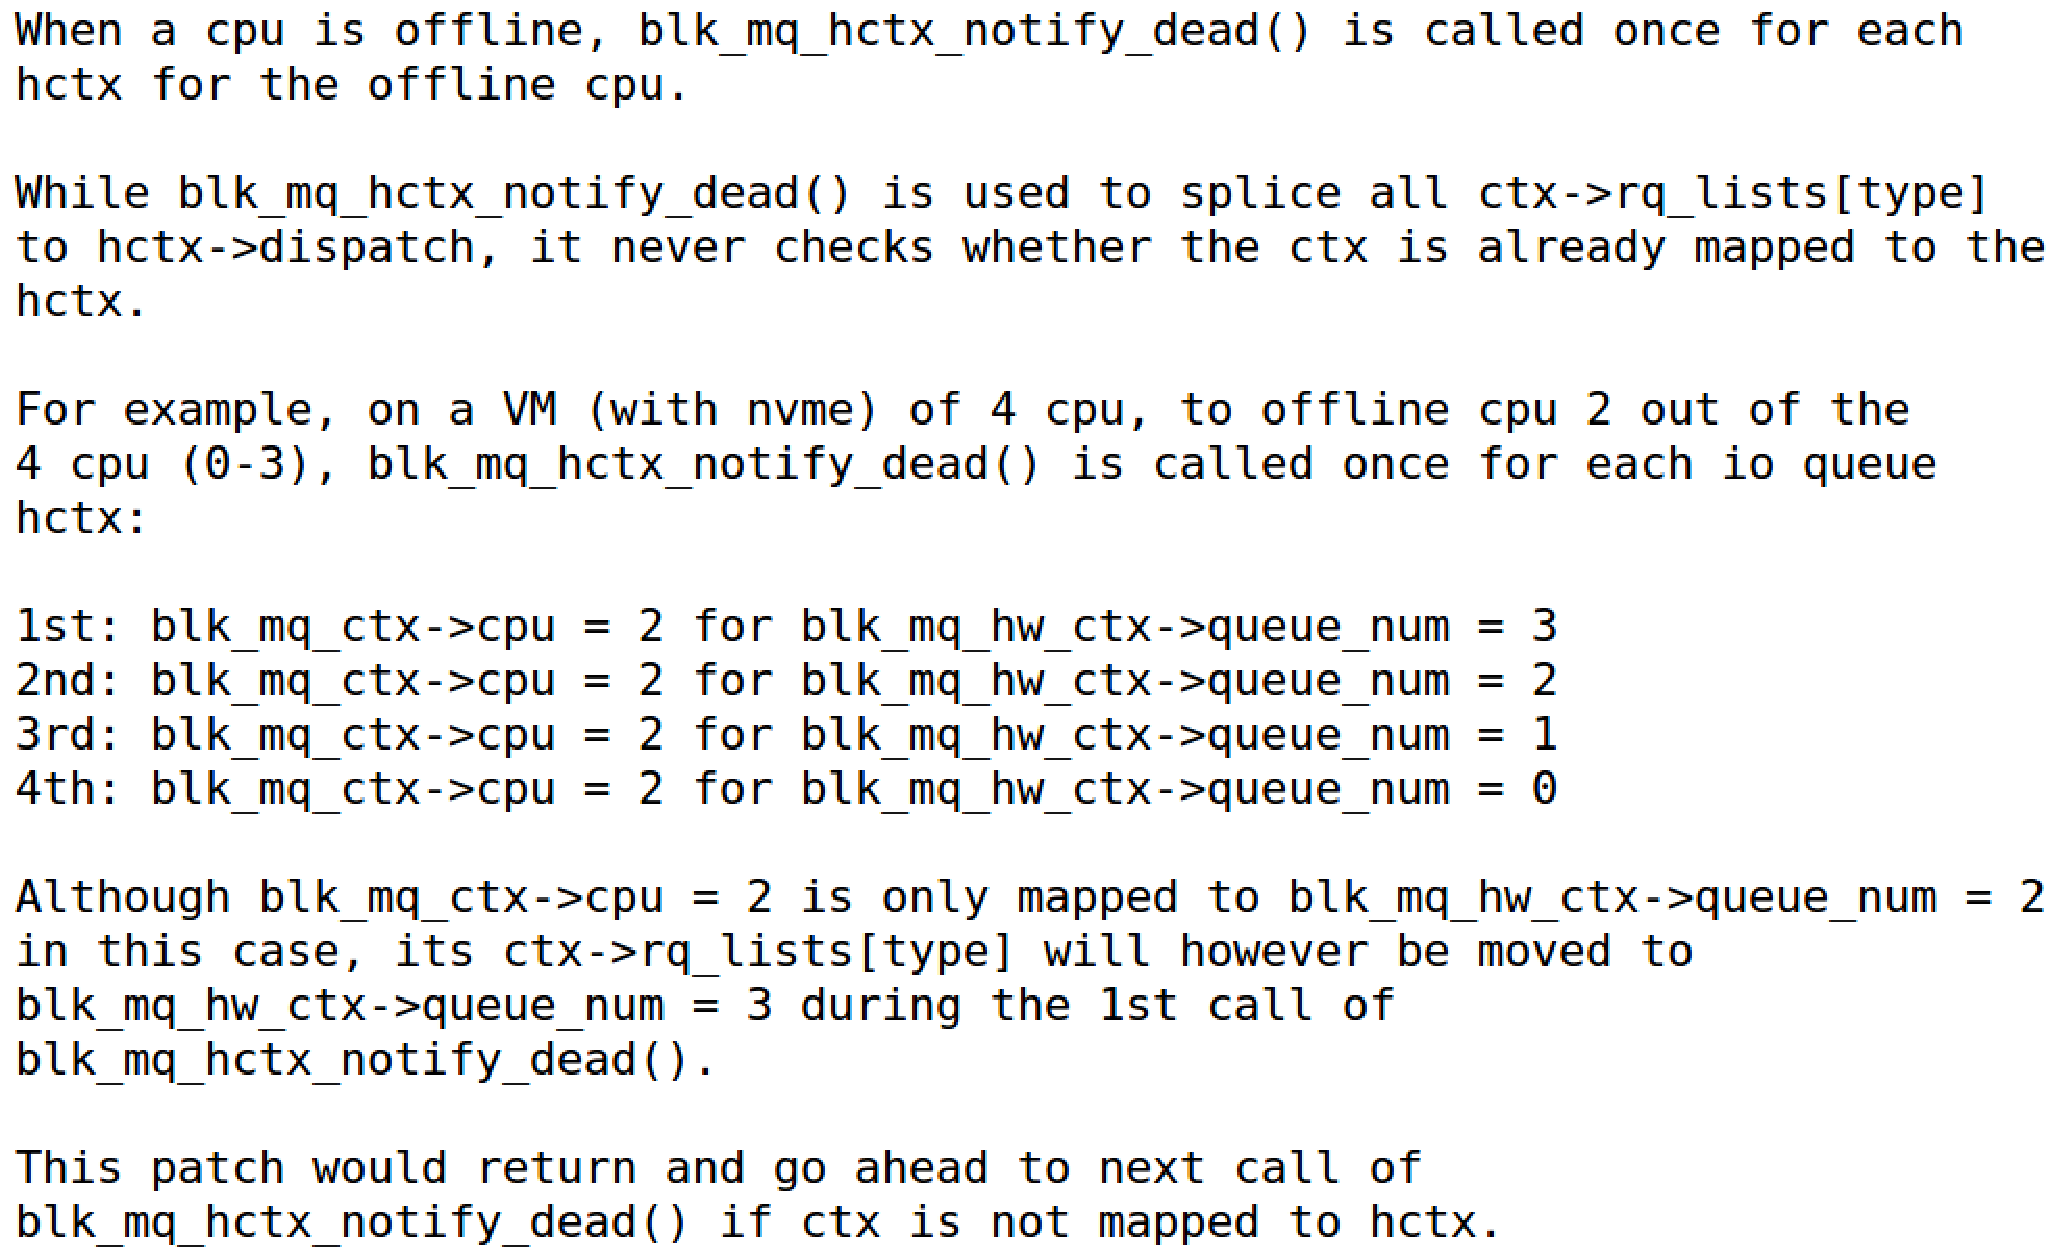
\includegraphics[width=0.6\linewidth]{figures/blk-cpu.pdf}
\end{figure}
\end{frame}


%------------------------------------------------

\section{Memory Hotplug 1/2}
\begin{frame}
\frametitle{Memory Hotplug 1/2}
Boot with:
\begin{itemize}
\item initial 2048MB memory
\item \textcolor{olive}{extra 4 slots} to hotplug memory up to extra 4096MB-2048MB=2048MB
\end{itemize}
\begin{block}{}

\# qemu-system-x86\_64 -machine accel=kvm -vnc :0 -smp 4 \textbackslash

\textcolor{red}{-m 2048M,\textbf{\textcolor{blue}{slots=4,maxmem=4096M}}} \textbackslash

-net nic -net user,hostfwd=tcp::5022-:22 \textbackslash

-kernel /home/user/linux/arch/x86\_64/boot/bzImage \textbackslash
	
-append "root=/dev/sda1 init=/sbin/init text" \textbackslash

-hda /home/user/img/boot.qcow2 \textbackslash

\textcolor{red}{-monitor stdio}

\textcolor{red}{QEMU 4.0.50 monitor - type 'help' for more information}

\textcolor{red}{(qemu)}
\end{block}
\end{frame}

%------------------------------------------------

\section{Memory Hotplug 2/2}
\begin{frame}
\frametitle{Memory Hotplug 2/2}
\begin{block}{}
\small
\textcolor{olive}{Before} memory hotplug: \newline
\# cat /proc/meminfo $|$ grep MemTotal \newline
MemTotal:\ \ \ \ \ \ \ \ \textcolor{red}{1972380 kB} \newline

To add 1024MB memory: \newline
\textbf{\textcolor{blue}{(qemu) object\_add memory-backend-ram,id=mem1,size=1024M}} \newline
\textbf{\textcolor{blue}{(qemu) device\_add pc-dimm,id=dimm1,memdev=mem1}} \newline

\# dmesg \newline
[   99.324281] Built 1 zonelists, mobility grouping on.  Total pages: 523480 \newline
[   99.324282] Policy zone: Normal \newline

\textcolor{olive}{After} memory hotplug (more 'memory$<$section$>$' available under \textbf{\textcolor{blue}{/sys/devices/system/memory/}}): \newline
\# cat /proc/meminfo $|$ grep MemTotal \newline
MemTotal:\ \ \ \ \ \ \ \ \textcolor{red}{3020956 kB}

\end{block}
\end{frame}

%------------------------------------------------

\section{PM Suspend 1/3}
\begin{frame}
\frametitle{PM Suspend 1/3}
\begin{itemize}
	\item To debug how each kernel component works during PM freezing, e.g., \textcolor{red}{unlike \textbf{\textcolor{blue}{jbd2}}, \textbf{\textcolor{blue}{o2hb\_thread}} does \textcolor{red}{NOT} freeze itself proactively}
\item To debug how each driver (e.g, nvme or virtio) works with PM suspend
\end{itemize}
\begin{block}{}

\# qemu-system-x86\_64 -machine accel=kvm -vnc :0 -smp 4 -m 4096M \textbackslash

-net nic -net user,hostfwd=tcp::5022-:22 \textbackslash

-kernel /home/user/linux/arch/x86\_64/boot/bzImage \textbackslash
	
-append "root=/dev/sda1 init=/sbin/init text" \textbackslash

-hda /home/user/img/boot.qcow2 \textbackslash

-device nvme,drive=nvme0,serial=deadbeaf1,num\_queues=8 \textbackslash

-drive file=/home/user/img/disk.qcow2,if=none,id=nvme0 \textbackslash

\textbf{\textcolor{blue}{-monitor stdio}} \textbackslash

\textcolor{red}{QEMU 4.0.50 monitor - type 'help' for more information} \textbackslash

\textcolor{red}{(qemu)}

\end{block}
\end{frame}

%------------------------------------------------

\section{PM Suspend 2/3}
\begin{frame}
\frametitle{PM Suspend 2/3}
\begin{block}{}
\scriptsize
\textbf{\textcolor{blue}{\# echo freeze $>$ /sys/power/state}} \ ---$>$ to suspend from VM \newline
\textbf{\textcolor{blue}{(qemu) system\_powerdown}} \ \ \ \ \ \ \ \ \ \ \ \  ---$>$ to resume from QEMU \newline

{\scriptsize
\# dmesg \newline
\textcolor{red}{[  \ 84.198422] PM: suspend entry (s2idle)} \newline
\textcolor{red}{[  \ 85.249993] Filesystems sync: 1.051 seconds} \newline
\textcolor{red}{[  \ 85.252942] Freezing user space processes ... (elapsed 0.001 seconds) done.} \newline
\textcolor{red}{[  \ 85.254433] OOM killer disabled.} \newline
\textcolor{red}{[  \ 85.254434] Freezing remaining freezable tasks ... (elapsed 0.000 seconds) done.} \newline
\textcolor{red}{[  \ 85.255212] printk: Suspending console(s) (use no\_console\_suspend to debug)} \newline
\textcolor{red}{[  \ 85.261298] sd 0:0:0:0: [sda] Synchronizing SCSI cache} \newline
\textcolor{red}{[  \ 85.283587] sd 0:0:0:0: [sda] Stopping disk} \newline
\textcolor{olive}{[  105.107310] sd 0:0:0:0: [sda] Starting disk} \newline
\textcolor{olive}{[  105.115072] nvme nvme0: 4/0/0 default/read/poll queues} \newline
\textcolor{olive}{[  105.261509] ata2.01: NODEV after polling detection} \newline
\textcolor{olive}{[  105.261896] ata1.01: NODEV after polling detection} \newline
\textcolor{olive}{[  105.265826] OOM killer enabled.} \newline
\textcolor{olive}{[  105.265827] Restarting tasks ... done.} \newline
\textcolor{olive}{[  105.273076] PM: suspend exit} \newline
\textcolor{olive}{[  107.172694] e1000: enp0s3 NIC Link is Up 1000 Mbps Full Duplex, Flow Control: RX}
}
\end{block}
\end{frame}

%------------------------------------------------

\section{PM Suspend 3/3}
\begin{frame}
\frametitle{PM Suspend 3/3}
\footnotesize
\begin{itemize}
\item Sample kernel warning at \textcolor{red}{kernel/irq/chip.c:210 irq\_startup+0xd6/0xe0}
\item Bug reported: \textcolor{red}{http://lists.infradead.org/pipermail/linux-nvme/2019-April/023234.html}
\item How I reproduce with QEMU: \textcolor{red}{http://lists.infradead.org/pipermail/linux-nvme/2019-April/023237.html}
\end{itemize}
\begin{figure}
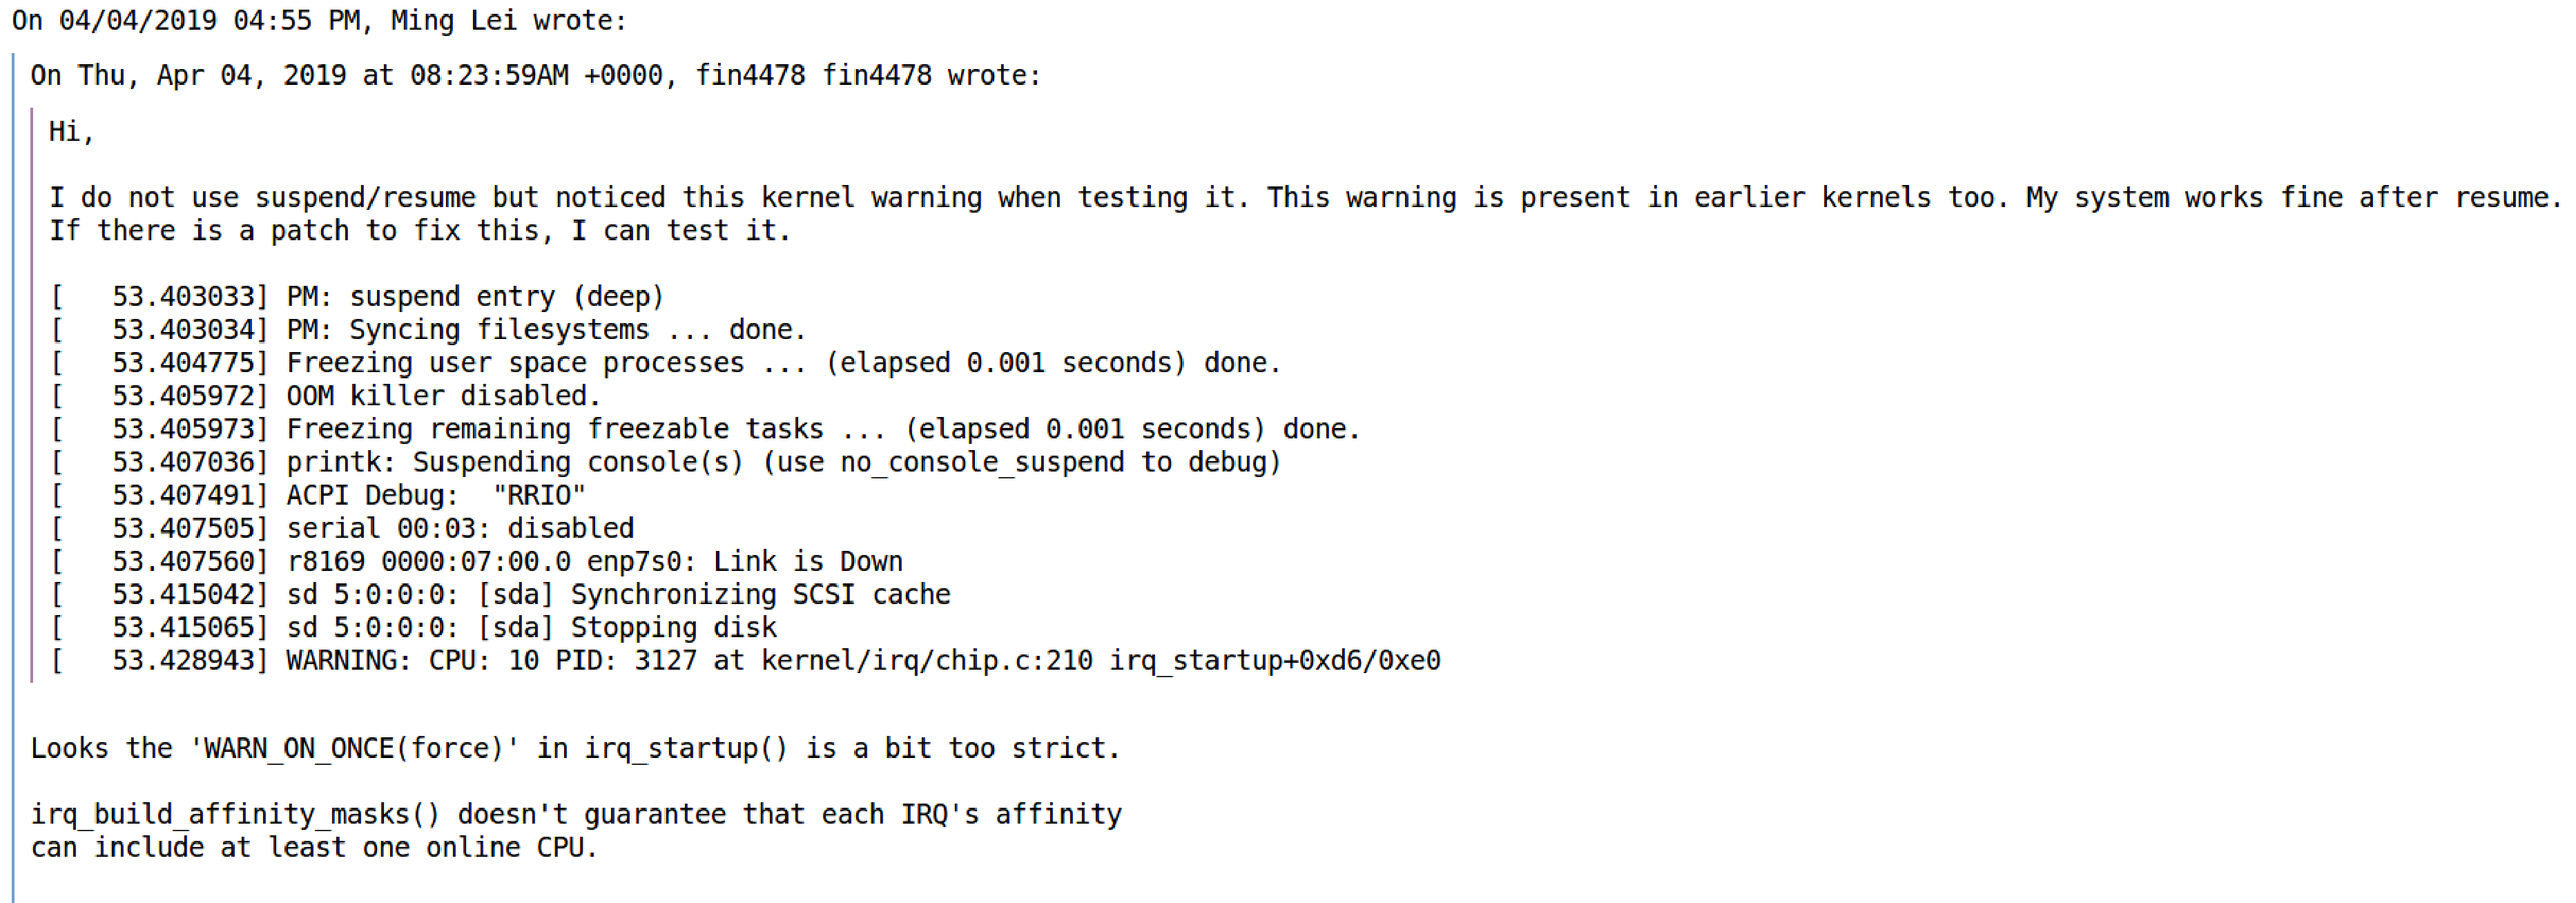
\includegraphics[width=1.0\linewidth]{figures/freeze.pdf}
\end{figure}
\end{frame}

%------------------------------------------------

\section{Do not always trust QEMU}
\begin{frame}
\frametitle{Do not always trust QEMU}
\footnotesize
\begin{itemize}
\item QEMU can have bug: \textcolor{red}{https://www.spinics.net/lists/linux-block/msg37936.html}
\item Fixed in QEMU commit \textbf{\textcolor{blue}{9d6459d21a6e ("nvme: fix write zeroes offset and count")}}
\end{itemize}
\begin{figure}
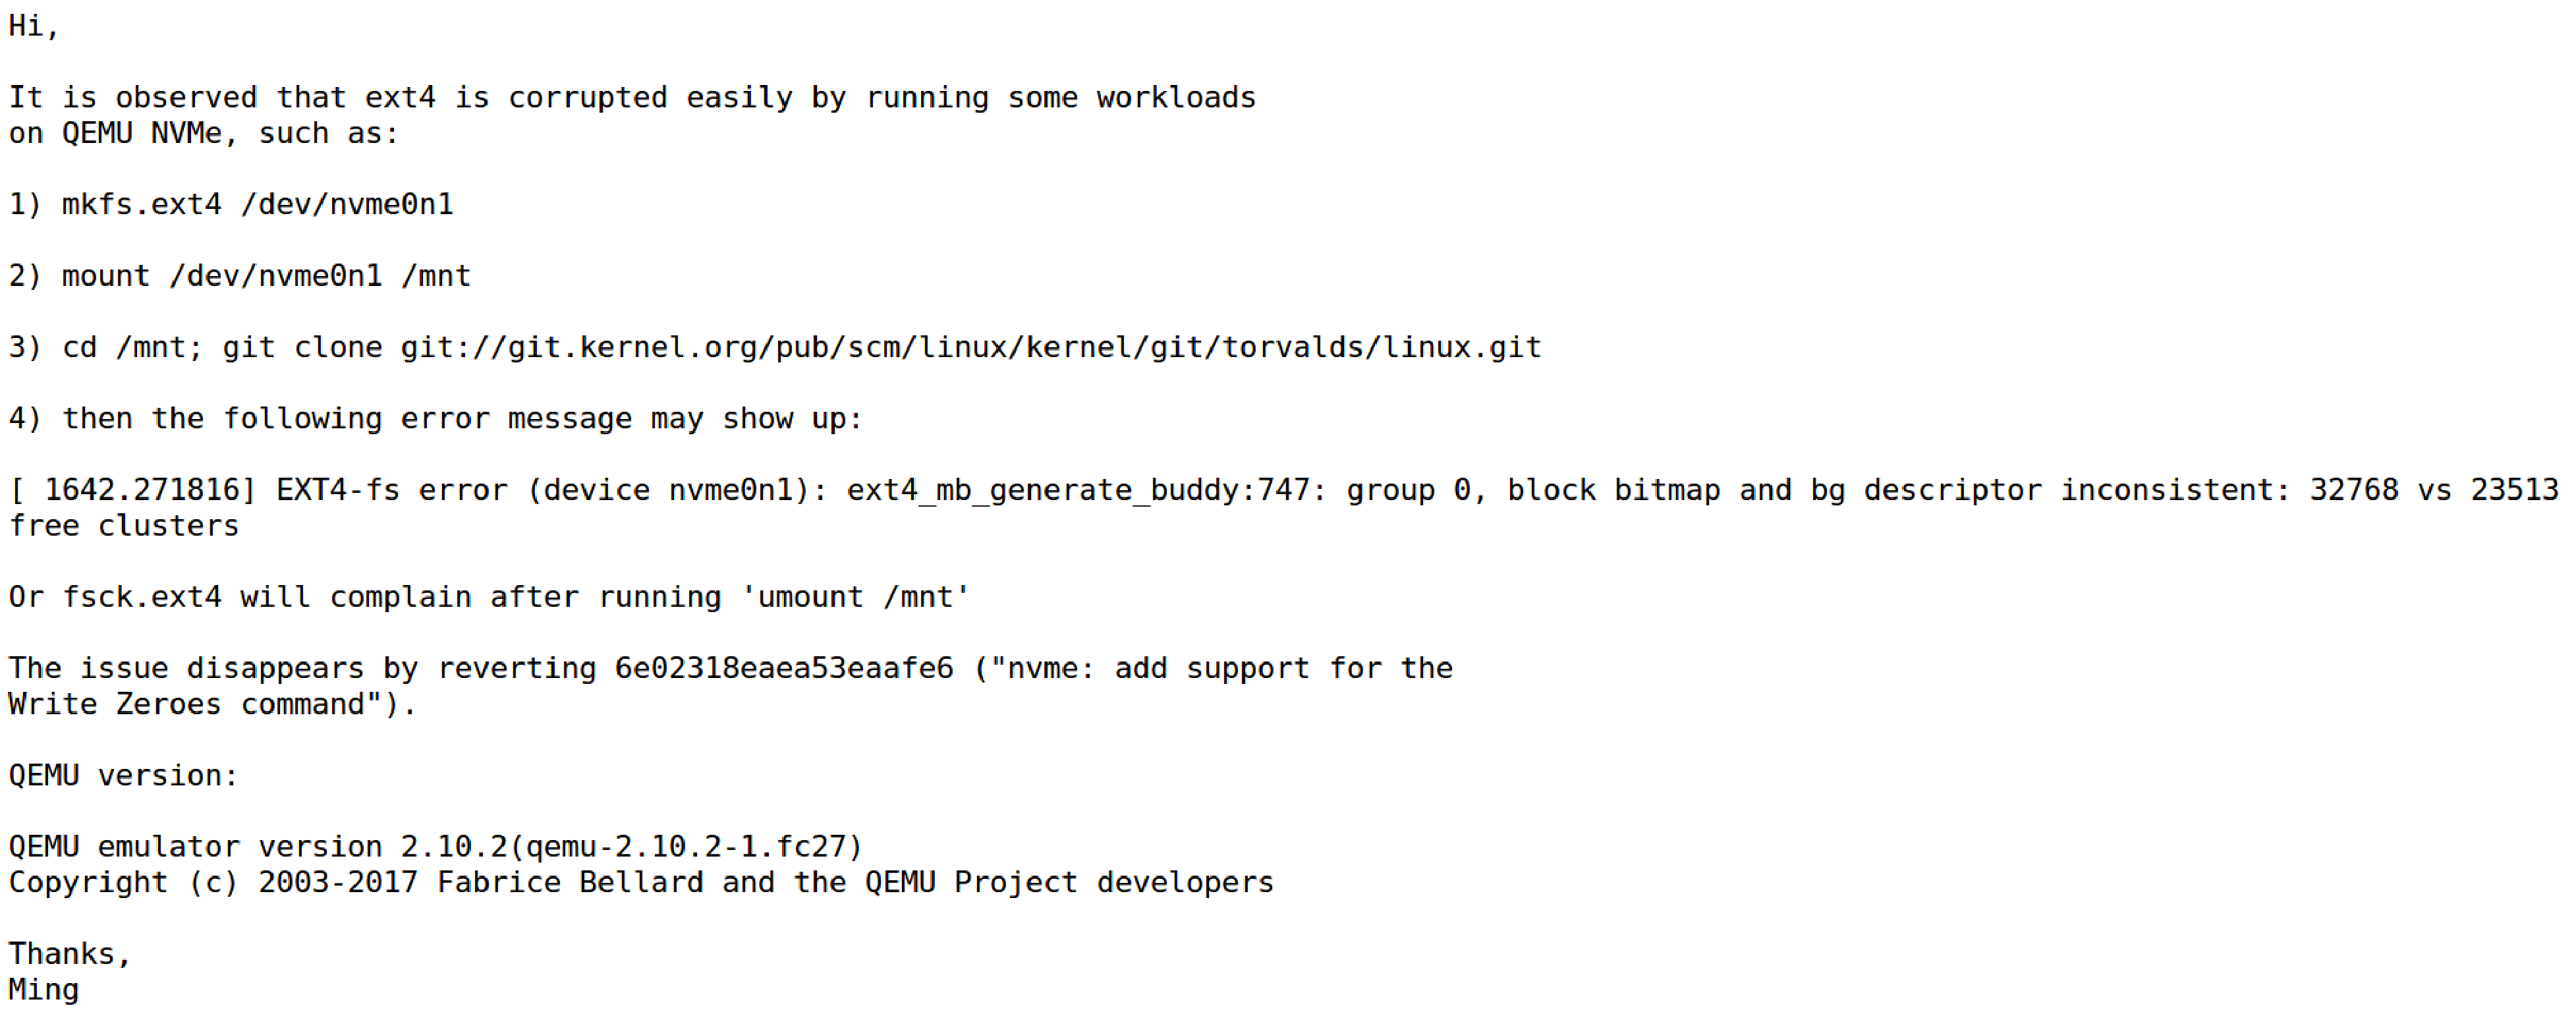
\includegraphics[width=1.0\linewidth]{figures/qemu-bug.pdf}
\end{figure}
\end{frame}

%------------------------------------------------

\section{Take-Home Message}
\begin{frame}
\frametitle{Take-Home Message}
{\Large How to \textbf{\textcolor{blue}{effectively}} setup \textbf{\textcolor{olive}{debug/study}} environment with QEMU:}
\begin{itemize}
\item {\Large \textcolor{red}{Build and run Linux kernel from host}}
\item {\Large \textcolor{red}{Use QEMU but not libvirt}}
\end{itemize}

\vspace{4 mm}

{\Large Components and Features to debug:}
\begin{itemize}
\item SCSI (megasas, lsi53c895a, virtio\_scsi), NVMe, NVDIMM
\item Virtio Block and Virtio Net
\item Ethernet Card (e1000e, e1000, e100, 8139cp, vmxnet3)
\item PCI Bus, PCIe Root Complex and PCIe Switch
\item BIOS (seabios), IOMMU (intel), PM Suspend
\item NUMA, Memory Hotplug, CPU Hotplug
\end{itemize}
\end{frame}

%----------------------------------------------------------------------------------------

\end{document} 
